% Options for packages loaded elsewhere
\PassOptionsToPackage{unicode}{hyperref}
\PassOptionsToPackage{hyphens}{url}
\PassOptionsToPackage{dvipsnames,svgnames,x11names}{xcolor}
%
\documentclass[
  authoryear,
  preprint,
  3p]{elsarticle}

\usepackage{amsmath,amssymb}
\usepackage{iftex}
\ifPDFTeX
  \usepackage[T1]{fontenc}
  \usepackage[utf8]{inputenc}
  \usepackage{textcomp} % provide euro and other symbols
\else % if luatex or xetex
  \usepackage{unicode-math}
  \defaultfontfeatures{Scale=MatchLowercase}
  \defaultfontfeatures[\rmfamily]{Ligatures=TeX,Scale=1}
\fi
\usepackage{lmodern}
\ifPDFTeX\else  
    % xetex/luatex font selection
\fi
% Use upquote if available, for straight quotes in verbatim environments
\IfFileExists{upquote.sty}{\usepackage{upquote}}{}
\IfFileExists{microtype.sty}{% use microtype if available
  \usepackage[]{microtype}
  \UseMicrotypeSet[protrusion]{basicmath} % disable protrusion for tt fonts
}{}
\makeatletter
\@ifundefined{KOMAClassName}{% if non-KOMA class
  \IfFileExists{parskip.sty}{%
    \usepackage{parskip}
  }{% else
    \setlength{\parindent}{0pt}
    \setlength{\parskip}{6pt plus 2pt minus 1pt}}
}{% if KOMA class
  \KOMAoptions{parskip=half}}
\makeatother
\usepackage{xcolor}
\setlength{\emergencystretch}{3em} % prevent overfull lines
\setcounter{secnumdepth}{5}
% Make \paragraph and \subparagraph free-standing
\makeatletter
\ifx\paragraph\undefined\else
  \let\oldparagraph\paragraph
  \renewcommand{\paragraph}{
    \@ifstar
      \xxxParagraphStar
      \xxxParagraphNoStar
  }
  \newcommand{\xxxParagraphStar}[1]{\oldparagraph*{#1}\mbox{}}
  \newcommand{\xxxParagraphNoStar}[1]{\oldparagraph{#1}\mbox{}}
\fi
\ifx\subparagraph\undefined\else
  \let\oldsubparagraph\subparagraph
  \renewcommand{\subparagraph}{
    \@ifstar
      \xxxSubParagraphStar
      \xxxSubParagraphNoStar
  }
  \newcommand{\xxxSubParagraphStar}[1]{\oldsubparagraph*{#1}\mbox{}}
  \newcommand{\xxxSubParagraphNoStar}[1]{\oldsubparagraph{#1}\mbox{}}
\fi
\makeatother


\providecommand{\tightlist}{%
  \setlength{\itemsep}{0pt}\setlength{\parskip}{0pt}}\usepackage{longtable,booktabs,array}
\usepackage{calc} % for calculating minipage widths
% Correct order of tables after \paragraph or \subparagraph
\usepackage{etoolbox}
\makeatletter
\patchcmd\longtable{\par}{\if@noskipsec\mbox{}\fi\par}{}{}
\makeatother
% Allow footnotes in longtable head/foot
\IfFileExists{footnotehyper.sty}{\usepackage{footnotehyper}}{\usepackage{footnote}}
\makesavenoteenv{longtable}
\usepackage{graphicx}
\makeatletter
\def\maxwidth{\ifdim\Gin@nat@width>\linewidth\linewidth\else\Gin@nat@width\fi}
\def\maxheight{\ifdim\Gin@nat@height>\textheight\textheight\else\Gin@nat@height\fi}
\makeatother
% Scale images if necessary, so that they will not overflow the page
% margins by default, and it is still possible to overwrite the defaults
% using explicit options in \includegraphics[width, height, ...]{}
\setkeys{Gin}{width=\maxwidth,height=\maxheight,keepaspectratio}
% Set default figure placement to htbp
\makeatletter
\def\fps@figure{htbp}
\makeatother

\usepackage{booktabs}
\usepackage{longtable}
\usepackage{array}
\usepackage{multirow}
\usepackage{wrapfig}
\usepackage{float}
\usepackage{colortbl}
\usepackage{pdflscape}
\usepackage{tabu}
\usepackage{threeparttable}
\usepackage{threeparttablex}
\usepackage[normalem]{ulem}
\usepackage{makecell}
\usepackage{xcolor}
\makeatletter
\@ifpackageloaded{caption}{}{\usepackage{caption}}
\AtBeginDocument{%
\ifdefined\contentsname
  \renewcommand*\contentsname{Table of contents}
\else
  \newcommand\contentsname{Table of contents}
\fi
\ifdefined\listfigurename
  \renewcommand*\listfigurename{List of Figures}
\else
  \newcommand\listfigurename{List of Figures}
\fi
\ifdefined\listtablename
  \renewcommand*\listtablename{List of Tables}
\else
  \newcommand\listtablename{List of Tables}
\fi
\ifdefined\figurename
  \renewcommand*\figurename{Figure}
\else
  \newcommand\figurename{Figure}
\fi
\ifdefined\tablename
  \renewcommand*\tablename{Table}
\else
  \newcommand\tablename{Table}
\fi
}
\@ifpackageloaded{float}{}{\usepackage{float}}
\floatstyle{ruled}
\@ifundefined{c@chapter}{\newfloat{codelisting}{h}{lop}}{\newfloat{codelisting}{h}{lop}[chapter]}
\floatname{codelisting}{Listing}
\newcommand*\listoflistings{\listof{codelisting}{List of Listings}}
\makeatother
\makeatletter
\makeatother
\makeatletter
\@ifpackageloaded{caption}{}{\usepackage{caption}}
\@ifpackageloaded{subcaption}{}{\usepackage{subcaption}}
\makeatother
\journal{Journal Name}

\ifLuaTeX
  \usepackage{selnolig}  % disable illegal ligatures
\fi
\usepackage[]{natbib}
\bibliographystyle{elsarticle-harv}
\usepackage{bookmark}

\IfFileExists{xurl.sty}{\usepackage{xurl}}{} % add URL line breaks if available
\urlstyle{same} % disable monospaced font for URLs
\hypersetup{
  pdftitle={A multi-scale story of the diffusion of a new technology: the web},
  pdfauthor={Emmanouil Tranos},
  pdfkeywords={diffusion, technologies, Web, digital},
  colorlinks=true,
  linkcolor={blue},
  filecolor={Maroon},
  citecolor={Blue},
  urlcolor={Blue},
  pdfcreator={LaTeX via pandoc}}


\setlength{\parindent}{6pt}
\begin{document}

\begin{frontmatter}
\title{A multi-scale story of the diffusion of a new technology: the
web}
\author[1]{Emmanouil Tranos%
\corref{cor1}%
}
 \ead{e.tranos@bristol.ac.uk} 

\affiliation[1]{organization={University of
Bristol},postcode={UK},postcodesep={}}

\cortext[cor1]{Corresponding author}

        
\begin{abstract}
Despite the broad consensus that differences in technological adoption
and sophistication can lead to uneven trajectories of local development
as new technologies can increase productivity and allow firms to
introduce new products and services, economic geographers have shied
away from exploring the diffusion of digital technologies across space
and time. This paper fills this gap by exposing the roles of different
spatial mechanisms in the diffusion of an intangible, digital technology
at very granular geographical scales. It does so by employing a novel
source of data and machine learning algorithms to model the active
engagement with Web during 1996-2012.
\end{abstract}





\begin{keyword}
    diffusion \sep technologies \sep Web \sep 
    digital
\end{keyword}
\end{frontmatter}
    

\section{Introduction}\label{sec-introduction}

Economic geographers were always interested in how new technologies and
innovations diffuse across space and time with the work of
\citet{hagerstrand1968innovation}, which demonstrated the importance of
communications as a mechanism for the diffusion of innovations, being
the most impactful. It was followed by various empirical studies -- see
for instance \citet{ormrod1990} and \citet{iso2005}. However, the torch
of exploring and modelling such diffusion processes had been passed to
other disciplines such as economics, business studies and sociology well
before the `cultural turn' of economic geography
\citep{perkins2005international}. A potential explanation of the lack of
geographical studies exploring the diffusion of new and, more
specifically for this paper, digital technologies across both space and
time can be attributed to the scarcity of relevant and granular enough
data, a problem also highlighted by \citet{iso2005} and
\citet{kemeny2011international}. As \citet{zook2022mapping} pointed,
digital activities are hardly ever captured in official data.

This paper offers such a contribution: an economic geography study
revealing the importance of spatial mechanisms for the diffusion of an
intangible, digital technology that is the Web in the UK at a high level
of spatial granularity during the 1996-2012 period. It does so by
employing a novel source of big data and machine learning algorithms to
model the \emph{active} engagement with Web during that period and tests
how different spatial and temporal mechanisms shaped its diffusion. This
paper also exemplifies how the combination of data sources and
state-of-the-art research methods which escape the traditional social
science domain can offer new lenses to geographical research regarding
the understanding of technological diffusion.

The motivation for this paper lies in the fact that there are various
stakeholders who are interested in knowing how new digital technologies
diffuse over space and time and use this knowledge to make predictions
about the diffusion of related future technologies. As per
\citet{leibowicz2016representing}, historical studies agree that
technologies diffuse differently in terms of times, rates, and
geographies and can be driven by related policies \citep{victor1993}.
\citet{meade2021modelling} highlight that a variety of actors have a
direct interest in gaining such knowledge including network equipment
suppliers, network operators, regulatory and local authorities. These
processes and their effects vary a lot across scales: although the
diffusion of a new technology might not be optimal at a local level, it
might be beneficial from a global perspective as it could lead to faster
diffusion to less advantaged places \citep{leibowicz2016representing}.
Despite the spatial heterogeneity of such diffusion mechanisms and the
policy relevance, there is a scarcity of studies analysing the diffusion
of new digital technologies at a detailed geographical level because of
the lack of detailed enough data and adequate research methods.

This gap becomes even more prominent if we consider the importance of
technology and its adoption in economic geography and macroeconomic
growth theories. Simply put, differences in technological adoption and
sophistication may lead to uneven development as new technologies can
increase productivity and allow firms to introduce new products
\citep{solow1957technical, aghion1990model, kemeny2011international}.
Linked to the subject of this paper, the Web -- and the active
engagement with this technology that is creating and maintaining instead
of just browsing a website -- can be considered as the underpinning
technology for the transformative process identified by
\citet{capello2024nexus} as the \emph{digital service economy}.
Importantly, the focus here is not the Web in general, but instead
commercial websites. After all, diffusion together with invention and
innovation are considered the pillars of technological change
\citep{das2022diffusion}. Findings from previous studies illustrated
that early engagement with digital technologies such as the Web led to
longstanding positive productivity gains for these regions that hosted
early adopters \citep{tranosuk}. Hence, obtaining a robust understanding
of the spatial diffusion mechanisms is crucial in mapping future
development trajectories.

Another line of motivation has to do with the intangible nature of the
Web and the debate about the footloose nature of digital technologies,
which contrary to several earlier general purpose technologies are
`light in weight' \citep{coyle1999weightless}. Following the seminal
work of \citet{gaspar1998information}, which demonstrated that
technological improvements in telecommunications lead to increased
demand for face-to-face communications and, consequently, enhance the
importance of cities, empirical studies from economic geography and
urban economics explored whether digital technologies substitute or
complement agglomeration externalities and spatial structure
\citep{kolko_death_2000, ioannides2008effect, tranos2021ubiquitous}.
With the exception of \citet{sinai2004geography}, who focused, among
other things, on web content and demonstrated that more such content is
available in larger markets, this strand of literature has been mostly
concerned with the spatiality of the Internet's hard and tangible
infrastructure and shied away from exploring the spatial dimensions of
one of the most distinct software layers of the Internet infrastructure,
the Web.

Technological diffusion, which is by definition an aggregated process,
can be discussed in parallel with individual adoption mechanisms. On the
one hand, \citet{rogers2010diffusion} identifies early adopter of new
technologies as `knowledgeable risk takers' and \citet{griliches1957} as
`profit maximisers' \citep{ding2010modeling}. Such individual agents are
rewarded because of their attitude towards new technologies and
innovations. On the other hand, \citet{perkins2011internet} attribute
diffusion to two processes: (i) epidemic-like mechanisms, which are
governed by distance, proximity and social interactions, and (ii)
economic mechanisms as new innovations are adopted by users as they
become more profitable, valueable and useful.

This paper focuses on the diffusion of the Web as new technology during
the 1996-2012 period. This was an exciting period for digital
technologies as it corresponds with the commercialisation of the
Internet and, consequently, its almost universal adoption. The reader is
reminded that it was only in 1994 when Netscape Navigator was
introduced, a year before Microsoft's Internet Explorer.\footnote{\url{https://www.theguardian.com/global/2015/mar/22/web-browser-came-back-haunt-microsoft}}
Also, only 9 per cent of UK's households had access to the Internet in
1998 \citep{ons2018}, the web included mostly static webpages, there
were no social media and web browsing involved exclusively a desktop PCs
as there were no smartphones \citep{tranosuk}. Hence, it is fair to say
that the study period captures the very early stages of the diffusion of
a new technology that is the Web until its maturity. The former is a key
point in the lifecycle of a new technology. Firstly, during this period
new technologies are expensive, crude and imperfect
\citep{rosenberg1994exploring, wilson201281}. A simple comparison
between Web 1.0 and Web 3.0 applications clearly illustrates this
\citep{tranos2020social}: while a static website facilitates one-way
information dissemination, a platform like \texttt{github} enables
cooperation between users and the creation of new information, meaning,
and even knowledge \citep{faraj2016special, barassi2012does}. During
this period the performance of a new technology is the main attraction
and not the cost to access and use it \citep{wilson2011lessons}. There
is a broader theoretical discussion in the literature about the early
adoption motives. As summarised by \citet{perkins2005international}, on
one hand, epidemic models highlight the role of interpersonal contacts
as a way for new technologies to diffuse. On the other hand, economic
models underline the importance of heterogeneity. Different firms have
different structures and business plans, which define the potential
economic returns of the adoption of a new technology and, therefore, the
choice to adopt a new technology becomes an individual option. From a
broader and evolutionary perspective, initial conditions are essential
for the creation and evolution of path-dependent technological
development trajectories \citep{neffke2011regions, simmie2014new}. This
argument is even more relevant when the focus is on digital technologies
because of the commonly found lag between investment and economic
returns as reflected in the Solow paradox
\citep{acemoglu2014return, brynjolfsson2018artificial}.

The data used here depict the active engagement with the Web as they
contain geolocated and time-stamped counts of commercial websites from
the UK. Instead of adopting metrics reflecting the passive engagement
with the Internet such as Internet adoption and speeds
\citep[e.g.][]{blank2018local, destefano2022fuzzy}, this paper observes
yearly counts of geolocated websites, which reflect the creation and
maintenance of websites. It needs to be highlighted here that although
there are various types of underpinning web technologies -- namely
markup, stylesheet, client- and server-side coding languages as well as
different web browsers and other related programming language -- the
focus here is on the diffusion of the Web in its totality. For a more
detailed and cross-country technological diffusion study, see
\citet{PAPAGIANNIDIS2015308}.

To analyse these data, a diverse set of methods are employed. Firstly,
cumulative adoption curves are estimated for the UK as a whole and for
the Local Authority Districts (LAD), illustrating, for the first time,
such S-shaped diffusion patterns for local areas. This system level
analysis also reveals insights about the volatility of the adoption of
the Web. Then, exploratory spatial data analysis offers some first
indications of the importance of the different spatial diffusion
mechanisms in shaping the diffusion of the Web in the UK. Importantly,
the analysis adopts two distinct geographical scales: the LAD and the
most detailed scale of UK census areas, the Output Areas (OA). Lastly, a
novel methodological framework based on Machine Learning (ML) algorithms
is developed to test the role of such mechanisms at these two scales.
The results reveal, for the first time, the importance of different
spatial diffusion mechanisms in the diffusion of an intangible, digital
technology at very granular geographical scales.

The structure of the paper goes as follows. Section~\ref{sec-litreview}
reviews the key concepts in the diffusion literature as well as relevant
empirical studies. Then, Section~\ref{sec-datamethods} describes the
data and methods used in this paper. The results of the different stages
of the analysis are presented in Section~\ref{sec-results}. The
discussion of the results and the conclusions of the paper are offered
in Section~\ref{sec-conclusions}.

\section{Literature review}\label{sec-litreview}

Geographical diffusion is a synthesis of different processes. On the one
hand, a purely spatial or, in other words, contagious processes can be
identified. Adjacency and, more broadly, distance are the key drivers of
diffusion. This perspective draws similarities with epidemics:
innovations just like pathogens spread because of contagion and,
consequently, proximity and exposure \citep{hivner2003facilitating}. On
the other hand, there is a hierarchical processes. According to this,
instead of a horizontal distance-based diffusion mechanism, the top-down
hierarchy of urban systems shapes technological diffusion. In reality,
the synthesis of these two processes better reflects how new
technologies diffuse over space \citep{morrill2020spatial}.

These ideas were firstly introduced by Torsten Hägerstrand and his
thesis entitled `Innovation Diffusion as a Spatial Process'
\citep{hagerstrand1968innovation}. Hägerstrand was the first to identify
diffusion as a geographical process. The starting point was the idea
that diffusion is based on passing information through social networks,
which themselves tend to be defined by geography. Hence, he identified a
`neighbourhood' mechanism of how information, and consequently,
innovation diffuse. He used agricultural innovations to test and model
his ideas using Monte Carlo simulations. Hägerstrand also incorporated
the role of hierarchy and how some phenomena maybe firstly adopted in
larger cities and then diffuse to second tier ones. This is a sequential
instead of a simultaneous process, which resembles the `lead-lag'
spatial acceleration effect in market research
\citep{bento2018time, PERES201091}. Hägerstrand is more widely known
though for highlighting the role time plays in the diffusion of
innovations: an early-pioneering period, a middle fast accelerating
period and a final saturation one \citep{morrill2020spatial}.

The temporal dimension was further explored by Everett Rogers and his
seminal work on `Diffusion of Innovations' \citep{rogers2010diffusion}.
Rogers being a sociologist focused not on the diffusion of innovations
over space and time, but instead on the adoption of new technologies and
innovations by individuals and the individual mechanisms that drive the
decisions behind adoption. He identified five groups of individuals
regarding their adoption speed: innovators, early adopters, early
majority, late majority and laggards. The key mechanism of diffusion and
adoption is communication and how knowledge is transferred within a
social system. All above approaches agree that diffusion and the
cumulative adoption of a new technology are represented by an S-shaped
line plot \citep{grubler1990rise}.

Schmidt's Law empirically illustrates a similar pattern. \emph{Core} and
usually highly agglomerated regions is where new technologies are
invented and commercially deployed \citep{grubler1990rise}. This is
where the first adopters tend to be based. Then, technologies spread to
the \emph{rim} and eventually to the \emph{periphery}. Although adoption
pace might be higher when new technologies finally arrive to the
periphery, the saturation levels there may never reach the ones in the
core because of the lack of infrastructure or other necessary
institutions \citep{leibowicz2016representing}.

\citet{grubler1990rise} effectively summarises the three key spatial
diffusion mechanisms: (i) the cumulative level of adoption follows an
S-shaped pattern just like purely temporal models; (ii) diffusion is
shaped by a hierarchical mechanism in a form of a centrifugal force:
from core to periphery; and (iii) diffusion is also shaped by distance
and proximity. These are the three mechanisms that the empirical
analysis in Section~\ref{sec-results} investigates.

The remaining of this section reviews empirical studies which analysed
the diffusion on new technologies over space and time. Although the
spatial dimension is present in most of the following studies, the level
of spatial detail is always more coarse than the one adopted in this
paper. \citet{beardsell1999spatial} studied the evolution of the
computer industry in 317 US metro areas during the 1977-1992 period
using employment data. Their analysis indicated that the relative size
distribution holds for urban computer employment and also urban
heterogeneity is essential in explaining this distribution. In a recent
study, \citet{bednarz2020pulled} focused on wind turbines and modelled
their spatial diffusion across 402 German regions during 1970-2015.
Their key finding is that local demand than local supply was the main
driving factor. \citet{haller2011determinants} employed firm panel data
for Ireland during 2003-2005 and illustrated that when firms are located
in a region or industry with high share of firms having a website, they
are more likely to have a website too.

At a global scale \citet{perkins2005international} explored whether the
diffusion rate of new technologies is driven by a latecomer advantage
and the engagement with the global economy via foreign direct
investments and trade. Their results illustrate that indeed latecomers
and developing countries experience diffusion of new technologies more
rapidly than early adopters and developed countries. At the same scale,
\citet{perkins2011internet} explored whether the adoption of previous
communication technologies that is mail, telegrams and telephones were
shaped by similar socioeconomic factors as the Internet. Their results
indicated common patterns regarding the drivers behind the adoption of
different communication technologies.

Turning to studies that share more technological and scalar similarities
with this paper, \citet{ding2010modeling} modelled the spatial diffusion
of mobile telecommunications across regions in China. Their analysis
indicated that socioeconomic characteristics are important determinants
of the timing, speed and the level of mobile diffusion within China.
Using data from a Hungarian online social network,
\citet{lengyel2020role} analysed its adoption and the churn at a very
granular spatial level. Their results were in agreement with the early
theoretical and empirical contributions reviewed here: assortativity,
urban scaling and distance are the key drivers of spatial diffusion.
\citet{bakher2013diffusion} compared different the growth curves as a
means to model diffusion of online shopping in Australia during the
1998-2009 period. At a global scale \citet{PAPAGIANNIDIS2015308}
modelled the diffusion of different web technologies and practices
across countries. Using similar but less extensive data as the one used
here, their analysis illustrated how the diffusion of different web
technologies and practices follow an S-shaped pattern as well as the
different diffusion rates of the different technologies and practices.

All in all, this paper tests whether the three distinct spatial
diffusion mechanisms shaped the diffusion of the Web in the UK at very
granular spatial scales from the Web's early stages onwards. The next
section discusses the empirical framework.

\section{Data and Methods}\label{sec-datamethods}

To capture the diffusion of the Web, a website density metric is
developed for two different geographical scales: the Local Authority
Districts (LAD) and the Output Areas (OA). The former is an
administrative unit and there are 374 LAD in the UK. The latter is the
smallest census-based geographical unit and there are c.~230,000 of them
in the UK. This methodological choice will allow the mapping of the
diffusion of web technologies and the assessment of the diffusion
mechanisms at these two very different spatial scales.

The counts of websites at these scales are calculated using data from
the Internet Archive\footnote{\href{See\%20https://archive.org/}{https://archive.org/}.}
and, specifically, the JISC UK Web Domain Dataset \citep{ukwebarchive}.
The Internet Archive is one of the most complete and oldest archive of
webpages in the world operating since 1996
\citep{ainsworth2011much, holzmann2016dawn}. It is a web crawler, which
discovers webpages by following the hyperlinks of every webpage it
archives. This dataset, which is curated by the British Library,
contains all the archived webpages from the UK country code top level
domain (ccTLD - .uk) from the 1996--2012 period. In essence, this is a
long list of 2.5 billion URLs of archived webpages including also the
archival timestamp.

Instead of using the whole .uk ccTLD, this paper focuses on its
commercial subset, the .co.uk second level domain (SLD). This choices
decrease the heterogeneity of the web data as such commercial websites
have specific aims: they are used to diffuse information, support online
transactions and share opinions
\citep{THELWALL2000441, blazquez2018big}. Although a UK company can
adopt a generic TLD such as .com and these cases escape the data used
here, such omissions should not affect the validity of the results given
the popularity of the .uk ccTLD \citep{tranosuk}: UK consumers prefer to
visit a .uk website when they are searching for products or services
\citep{hope}; and anecdotal evidence indicates that during the first
half of 2000, three .co.uk domains were registered every minute
\citep{oecd_coms}. Importantly, previous studies illustrated that .co.uk
is the most popular UK SLD \citep{tranosuk}.

The text from these webpages was scanned using a regular expression
(regex) to identify strings of text which resemble UK postcodes and one
fifth of them included a mention to a postcode \citep{BL2013geo}. This
information allows the geolocation of the data and the creation of the
LAD and OA counts.

The data cleaning process includes an aggregation step, through which
the archived webpages are aggregated to the parent websites. This
website reconstruction process lend itself to the construction of
\emph{website} instead of \emph{webpage} density metrics. Websites tend
to represent specific organisations or entities, and, arguably, are more
meaningful observational units than webpages, which can ignore the
upstream dependency of the website they belong to. Based on the
following example, all three webpages are part of the same website
(\url{http://www.website.co.uk}). Only the overall website and not the
nested webpages are considered for the counts as otherwise the density
metrics would have been biased towards large, place specific, websites.

\begin{itemize}
\item
  \url{http://www.website.co.uk/webpage_a} B15 2TT
\item
  \url{http://www.website.co.uk/webpage_b} BS8 1TH
\item
  \url{http://www.website.co.uk/webpage_c} B15 2TT
\end{itemize}

\noindent What is challenging is that this aggregation approach, which
has been used elsewhere \citep{tranosuk, shoreditch} may lead to
websites with multiple postcodes. As per the above example,
\href{http://www.website.co.uk}{www.website.co.uk} includes two unique
postcodes: B15 2TT and BS8 1SS. The distribution of the number of
postcodes per website for 2000 is presented in Table \ref{f2000}, which
illustrates a wide range. At the left end of the distribution, there are
websites anchored to a unique location (72\% of all the reconstructed
websites in 2000), which may represent a small company with a single
trading location. At the right end, there are websites with thousands of
different postcodes. Considering the time period of the analysis, such
cases can represent directories which used to be popular in the
pre-search engines early times of the commercial Internet as well as
real estate websites \citep{tranosuk}.

The analysis is firstly conducted on websites, which only contain one
unique postcode. As a robustness check, the analysis is replicated for
an extended subset of websites, which include up to 10 unique postcodes
to capture commercial websites which point to multiple locations. They
are geolocated by equally attaching them to these locations. This
extended sample includes 94 percent of all the archived websites in
2000.

\begin{table}

\caption{Number of unique postcodes per .co.uk website, 2000.\label{f2000}}
\centering
\begin{tabular}[t]{lrrr}
\toprule
Postcodes & F & F (\%) & Cummulative F\\
\midrule
(0,1] & 41,596 & 0.718 & 0.718\\
(1,2] & 6,451 & 0.111 & 0.830\\
(2,10] & 6,163 & 0.106 & 0.936\\
(10,100] & 2,975 & 0.051 & 0.988\\
(100,1000] & 646 & 0.011 & 0.999\\
\addlinespace
(1000,10000] & 62 & 0.001 & 1.000\\
(10000,100000] & 4 & 0.000 & 1.000\\
\bottomrule
\multicolumn{4}{l}{\rule{0pt}{1em}\textit{Source: } Tranos et al. 2021}\\
\end{tabular}
\end{table}

Another data cleaning step deals with some extreme outliers. Figure
\ref{correct} plots the website counts for the top 1000 postcodes. Some
obvious outliers can be observed for the 2002-2006 period for a handful
of postcodes, which can be attributed to link farms \citep{BL2013links}.
The website counts for these postcodes (SE24 9HP, CV8 2ED, GL16 7YA, CW1
6GL, M28 2SL, DE21 7BF), which in 2004 or 2005 had more than 1000
websites pointing to them, were replaced with predicted values based on
a simple panel regression model with postcode fixed effects and yearly
dummy variables. These postcodes refer to a residential area with a
small park in South London, residential areas outside Warwick and
Manchester, a rural area in the south border of England and Wales and
small business parks in Crew and Derby. Hence, it is difficult to
believe that these postcodes genuinely hosted such a large amounts of
websites, which were later extensively declined. To put the magnitude of
the data imputation into perspective, this process affected 6 out of the
557,808 postcodes included in the data. As the Section~\ref{sec-results}
illustrates, this led to a small increase of the model predictive power.

\begin{figure}[H]

{\centering 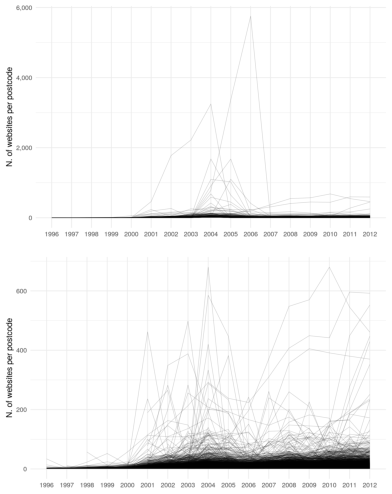
\includegraphics[width=1\textwidth,height=0.7\textheight]{tranos2023_files/figure-pdf/unnamed-chunk-2-1.pdf}

}

\caption{\label{correct}Yearly website counts per postcode (top 1000)
before (top) and after (down) data imputation}

\end{figure}%

To create the website density metric, the yearly website counts at the
LAD level are standardised by the number of firms in LAD to avoid biases
associated with LAD hosting a large number of firms. Given that there is
no such readily available statistic for the OA, the actual OA level
counts are used. However, because of the the consistent spatial
definition of OA (they host 40-250 households),\footnote{\url{https://www.ons.gov.uk/methodology/geography/ukgeographies/statisticalgeographies}}
website counts in OA are interpreted as a density metric too.

These website density metrics are used for the three different stages of
the analysis. Firstly, a system-level analysis explores how the
diffusion of web technologies in the UK fits with the well-established
S-curve of cumulative adoption. To do so, the following logistic
function (Equation \ref{eq:s}) is estimated for the whole of the UK and
for each LAD separately:

\begin{align}
y = k /(1 + e^{-(t-t_{o})})\label{eq:s}
\end{align}

\noindent \(k\) is the asymptote or, in other words, the saturation
level, \(b\) the overall growth rate, and \(t_{0}\) the \emph{inflection
point} of maximum growth at \(k/2\), where the logistic function is
symmetrical \citep{wilson201281}. The \(t_0\) of each LAD is compared
against the \(t_0\) of the UK to delineate whether a LAD reached that
point faster or slower than the country average. Importantly, an
accuracy criterion was imposed and only LAD with \(R^2 > 0.9\) were
included in this analysis. To estimate Equation \ref{eq:s} a
self-starting logistic growth model was employed using the \texttt{nls}
and \texttt{SSlogis} functions in \texttt{R}. This logistic growth model
depicts the initial period of slow diffusion of a new technology, which
is followed by the fast, exponential growth stage to then eventually
slow down and saturate \citep{wilson201281, grubler1999dynamics}.

The system-level analysis also focuses on the volatility of the web
adoption to depict places with high concentration of early adopters and,
equally, latecomers. To do so, the change of the ranking of the UK LAD
over time is plotted and discussed. Both the S-curve and the volatility
analysis focus only on LAD as the very large number of OA would have
made such analysis difficult to visualise and interpret.

Next, exploratory spatial data analysis depicts whether the two main
drivers of spatial diffusion -- namely neighbourhood and hierarchy --
underpin the diffusion of the Web in the UK. To capture the former and
following \citet{ding2010modeling} the Moran's I and the Local Index of
Spatial Association (LISA) are estimated for the website density. To
address the hierarchy mechanism, the Gini coefficient -- an established
metric of inequality -- is calculated. All the above are computed and
plotted longitudinally both for the LAD and the OA.

Lastly, a modelling framework is developed to test the above diffusion
mechanisms. The overarching aim is to build a model that can test how
well these mechanisms can predict website density:

\begin{align}
Website\,Density_{t} \sim Hierarchy_{t-1} + Neighbourhood_{t-1} + S-curve_{t}\label{eq:rf.generic}
\end{align}

\noindent Equation \ref{eq:rf.generic} is estimated using Random Forest
(RF). This is a popular ML algorithm for both regression and
classification problems \citep{biau2012analysis}. It was introduced by
\citet{breiman2001random} and has become a go-to data science tool. RF
can effectively handle skewed distributions and outliers, model
non-linear relationships, require minimal hyperparameter tuning, exhibit
low sensitivity to these parameters, and have relatively short training
times \citep{Caruana2008, liaw2002classification, yan2020using}. These
attributes match well with the website density data characteristics
including skewness especially for the OA. Also, the large data size
(c.~230k data points for each of the 17 years) calls for fast training
times. Importantly, RF predictions tend to be more accurate than those
from single regression trees and outperform Ordinary Least Squares in
out-of-sample predictions, even with moderate-sized training data and a
small number of predictors
\citep{mullainathan2017machine, athey2019machine, sulaiman2011intelligent, pourebrahim2019trip, biau2012analysis}.

RF is a tree-based ensemble learning algorithm
\citep{breiman2001random}. It begins by generating random samples of the
training data, which are then used to grow regression trees to predict
the dependent variable. Data points and predictors are randomly sampled
for the different trees. The trees are trained in parallel using their
own bootstrapped samples of the training data. A crucial feature of RF
is their ability not to overfit, meaning they can generalize well to
unseen test data. While each tree may overfit individually, the ensemble
of trees does not because the errors of individual trees are averaged,
reducing the overall variance and preventing overfitting
\citep{last2002improving}. For regression problems, RF predictions are
made by averaging the predictions of all decision trees.

RF have been widely employed to address regression research problems.
\citet{pourebrahim2019trip} combined a spatial interaction modelling
framework with ML algorithms including RF to predict commuting flows in
New York City. \citet{sinha2019assessing} advocated for adopting spatial
ensemble learning approaches, such as RF, to model spatial data with
high autocorrelation and heterogeneity. \citet{creditspatial} predicted
employment density in Los Angeles using spatially explicit RF.
\citet{guns2014recommending} used RF to build a recommendation system
for research collaborations. \citet{ren2019predicting} trained RF to
predict the socio-economic status of cities using various online and
mobility predictors. \citet{tranos2023using} utilised hyperlinks data
and RF to make out-of-sample predictions of interregional trade.
\citet{zhou2023geography} employed such a framework to assess whether
key predictors of obesity differ across English cities.

\section{Results}\label{sec-results}

\subsection{System-level analysis}\label{system-level-analysis}

\begin{figure}[H]

{\centering 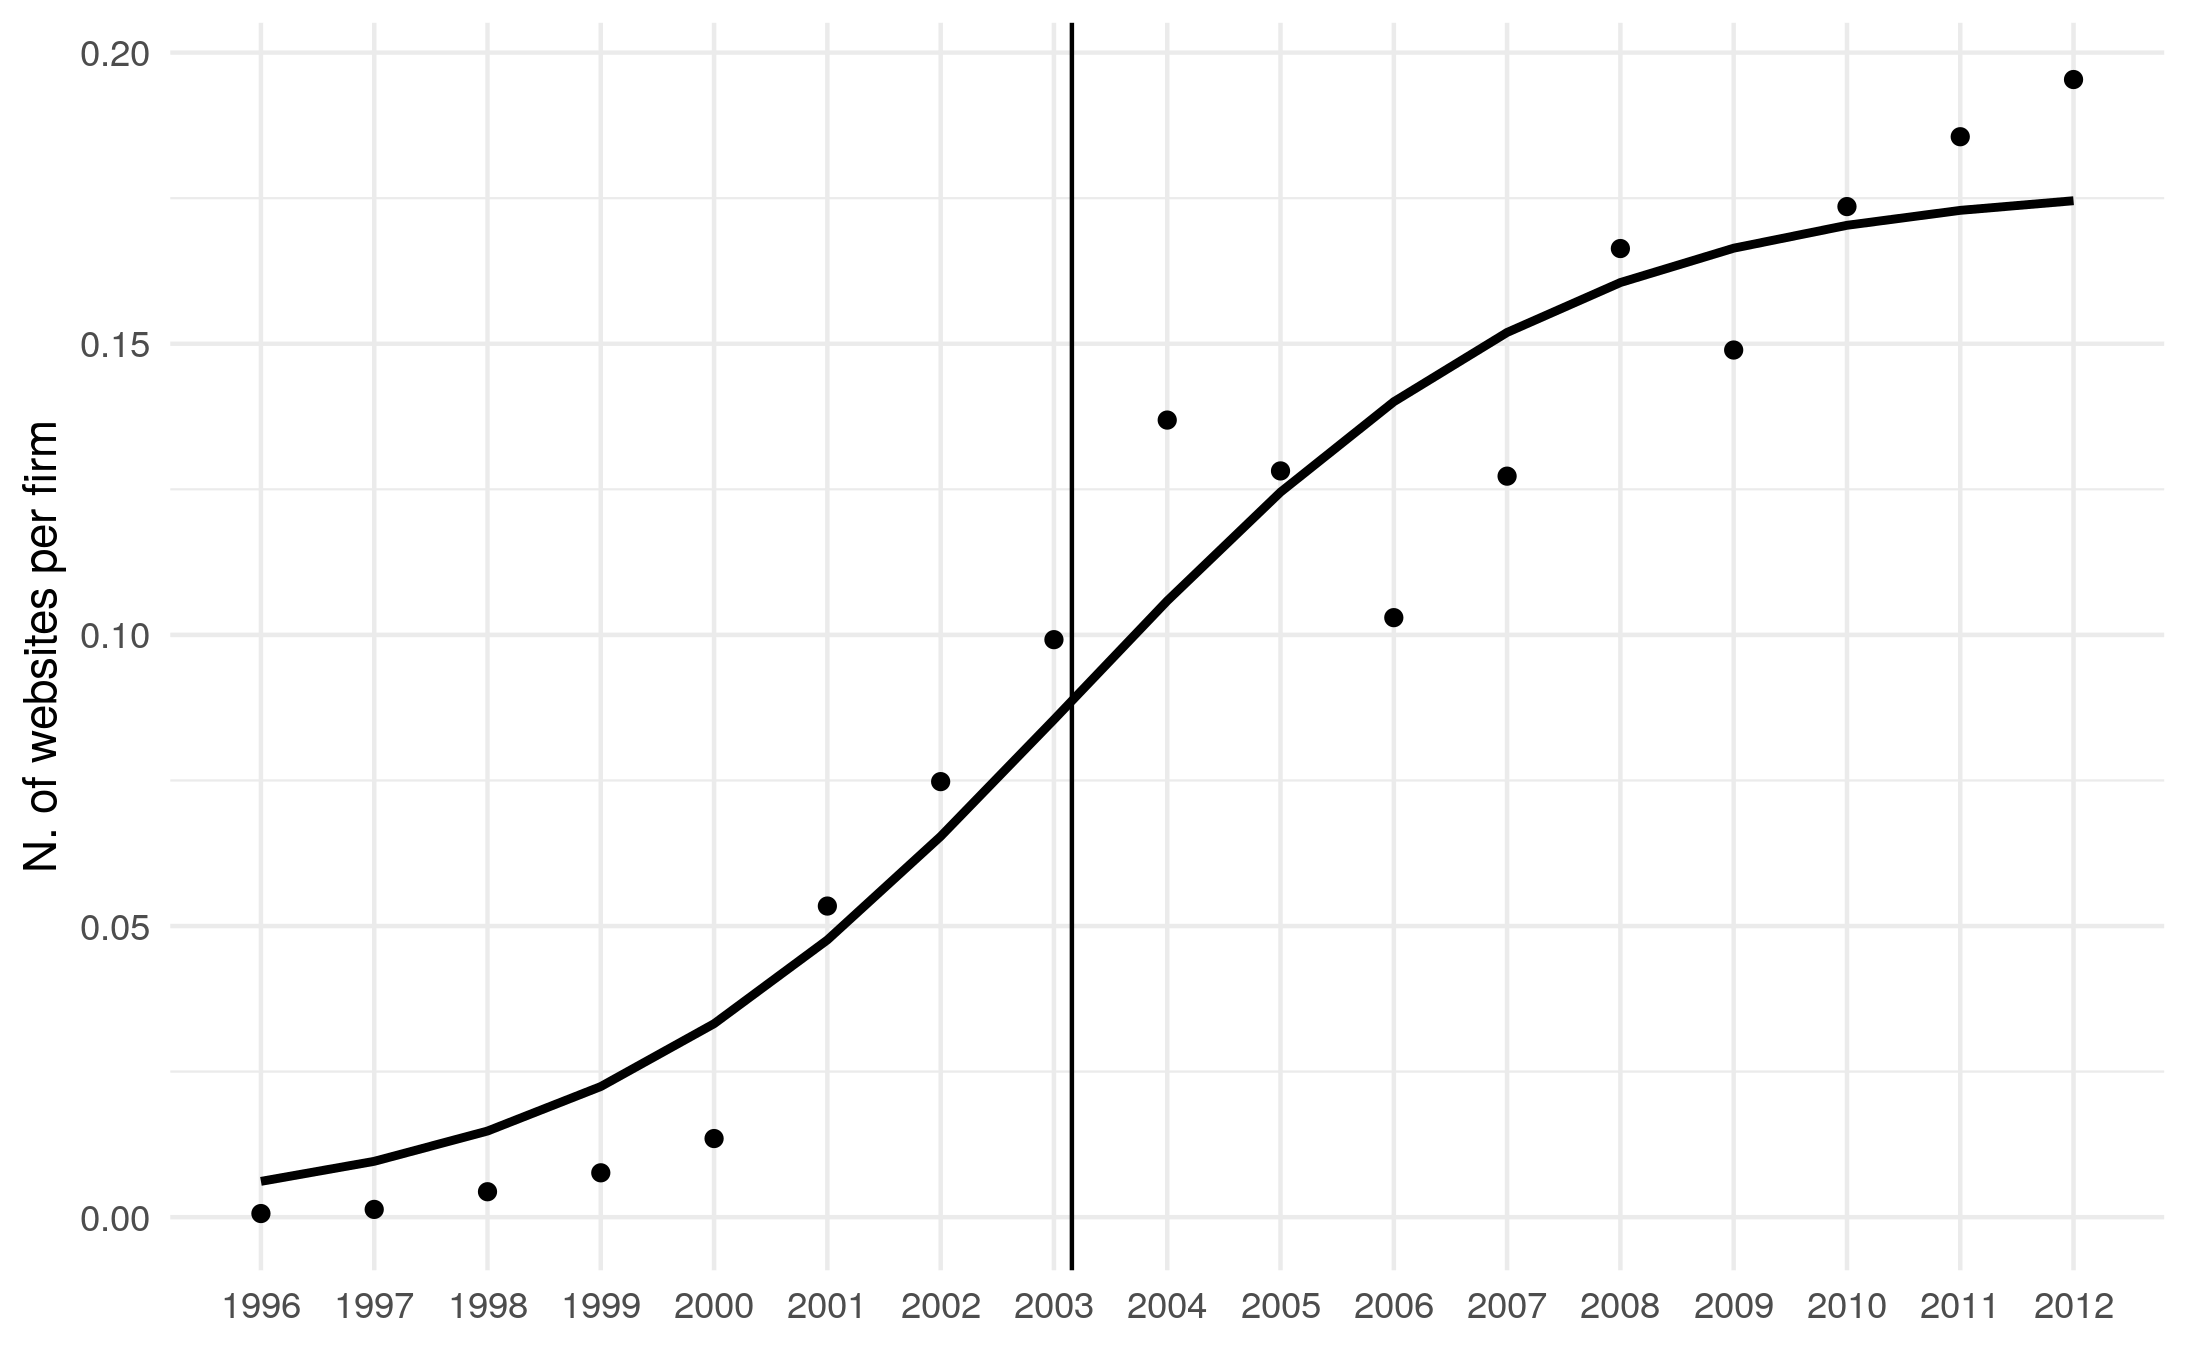
\includegraphics[width=1\textwidth,height=\textheight]{../../outputs/s/s_uk_per_firm.png}

}

\caption{\label{s_uk}Grwoth curve, UK}

\end{figure}%

Figure \ref{s_uk} plots the cumulative adoption of the Web in total in
the UK during the 1996-2012 period. Not surprisingly, the cumulative
adoption is well represented by a curve that resembles the figure S. The
vertical line around year 2003 illustrates the point where the modelled
cumulative adoption is equal to 50\% of the maximum. This \(t_0\)
\emph{inflection} point signals the maximum adoption speed and is used
here to determine whether a UK LAD reached that inflection point earlier
or later than the UK average. Specifically, the S curve and the
inflection point are estimated for every LAD individually and then
compared against the UK average. LAD that reached their inflection point
earlier than the country average are labelled as \emph{fast} and the
rest as \emph{slow}. Figure \ref{s_map} maps this pattern. There is a
clear high concentration of fast adopting LAD in the South and East of
England as expected. However, there is also such a concentration in
Wales, Scotland and the North West of England. At a more detailed level,
there are some expected examples of LAD with relevant industrial
backgrounds delineated as fast: the City of London, a world-renowned
cluster of finance industries \citep{cook2007role}, and Reading, a town
with high-tech service industries in proximity to London and its main
airport, Heathrow \citep{england2005polynet}. However, there are also
LAD which were expected to appear as fast -- e.g.~Hackney in central
London and Bristol, a well-established creative cluster
\citep{oatley1999cultural, bassett2002cultural} -- but were delineated
as slow. Nevertheless, there is obvious spatial clustering of fast and
slow LAD. Importantly, out of the ten fastest LAD, nine were located in
the South East of England and London and one in Cambridge (see Table
\ref{table.s.lads} in the Appendix). The above observations remain
almost unchanged when the analysis includes websites with up to 10
unique postcodes -- see Figures \ref{s_uk10} and \ref{s_map10} in the
Appendix -- advocating towards the robustness of the analysis.

\begin{figure}[H]

{\centering 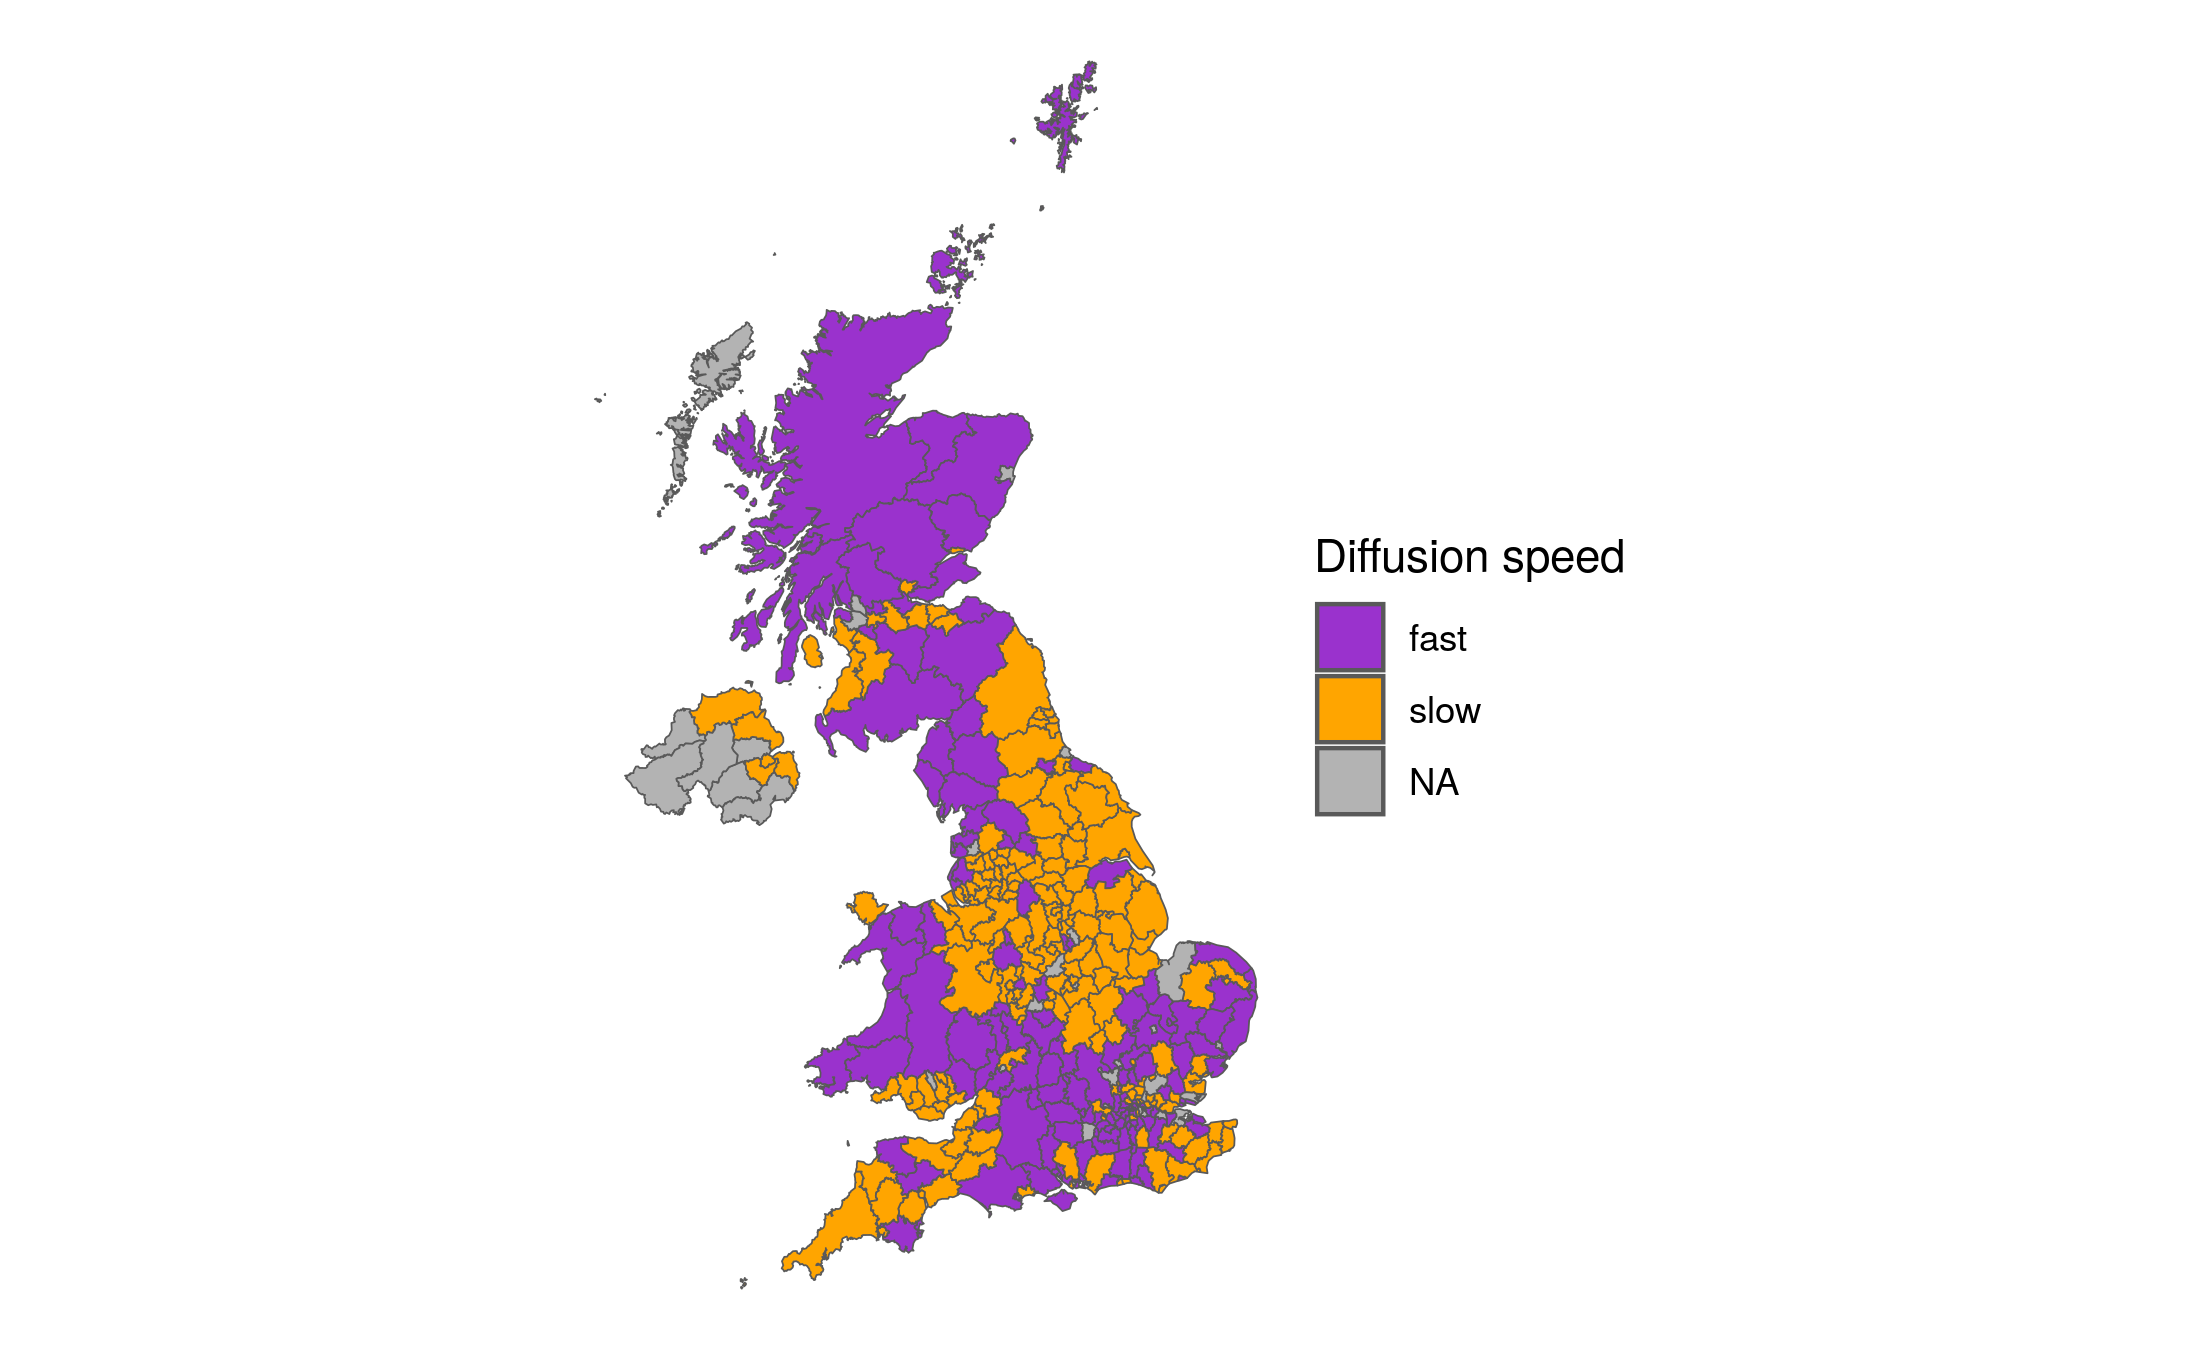
\includegraphics[width=1\textwidth,height=\textheight]{../../outputs/s/speed_map.png}

}

\caption{\label{s_map}LAD adoption rates}

\end{figure}%

The S-curves of the cumulative adoption of Web in the UK in total and in
the UK LAD demonstrate a pattern well aligned with all previous studies
discussed in Section~\ref{sec-litreview}. Importantly, the above
findings are in line with previous studies exploring the diffusion of
web technologies \citep{PAPAGIANNIDIS2015308}, social media
\citep{lengyel2020role} and online shopping \citep{bakher2013diffusion}.
Similar to \citet{beardsell1999spatial}, who analysed the spatial
evolution of computer industry employment across 317 US metro areas,
spatial heterogeneity is evident in the diffusion speed when the scale
of analysis is as detailed as the LAD. Importantly, no previous studies
estimated such cumulative adoption curves for areal units as small as
the UK LADS.

The next step assesses the stability and volatility of the LAD in terms
of their adoption of web technologies. As highlighted in the literature
\citep{risk_perceptions}, different agents have different perceptions
about and levels of acceptance of the risks and the potential economic
returns associated with the adoption of new technologies -- see for
instance the seminal work of \citet{venkatesh2000theoretical}. To reveal
such aggregated patterns, Figure \ref{rank} plots the ranking of UK LAD
based on website density. To decrease noise, the average ranking of
1996-1998 and 2010-2012 is plotted instead of the individual years. The
colours depict the 5th and 95th percentile of the absolute difference of
the LAD ranking between 1996-1998 and 2010-2012. While there are quite a
few obvious cases of LAD that maintained their position between the
beginning and the end of the study period both at the top or at the
bottom of the hierarchy, there are also quite a few LAD that changed
drastically their position. Some of these LAD enjoyed a process that at
the first instance looks like \emph{leapfrogging} since they managed to
jump at the top of the hierarchy despite their slow start. There is
extensive literature regarding the potential benefits of technological
leapfrogging. The underpinning argument is that latecomers can adopt and
benefit from new technologies that have been developed elsewhere without
incurring the hefty initial R\&D costs \citep{teece2008firm}. Although
the leapfrogging literature does not pay much attention to cities and
regions \citep{yu2018sustainability}, previous research highlighted the
long term and sustained productivity benefit of the early adopters of
web technologies in the UK \citep{tranosuk}. So, although the LAD system
is volatile, it is not clear whether the LAD with high concentration of
late adopters will gain any latecomer-related benefits in a way similar
to countries experiencing technological leapfrogging. Still, the
opportunity to catch up that \citet{perkins2005international}
illustrated at the country level, is also visible at the much more
detailed LAD scale. As previously, this is consistent with including
websites with up to 10 postcodes (see Figure \ref{rank10}).

\begin{figure}[H]

{\centering 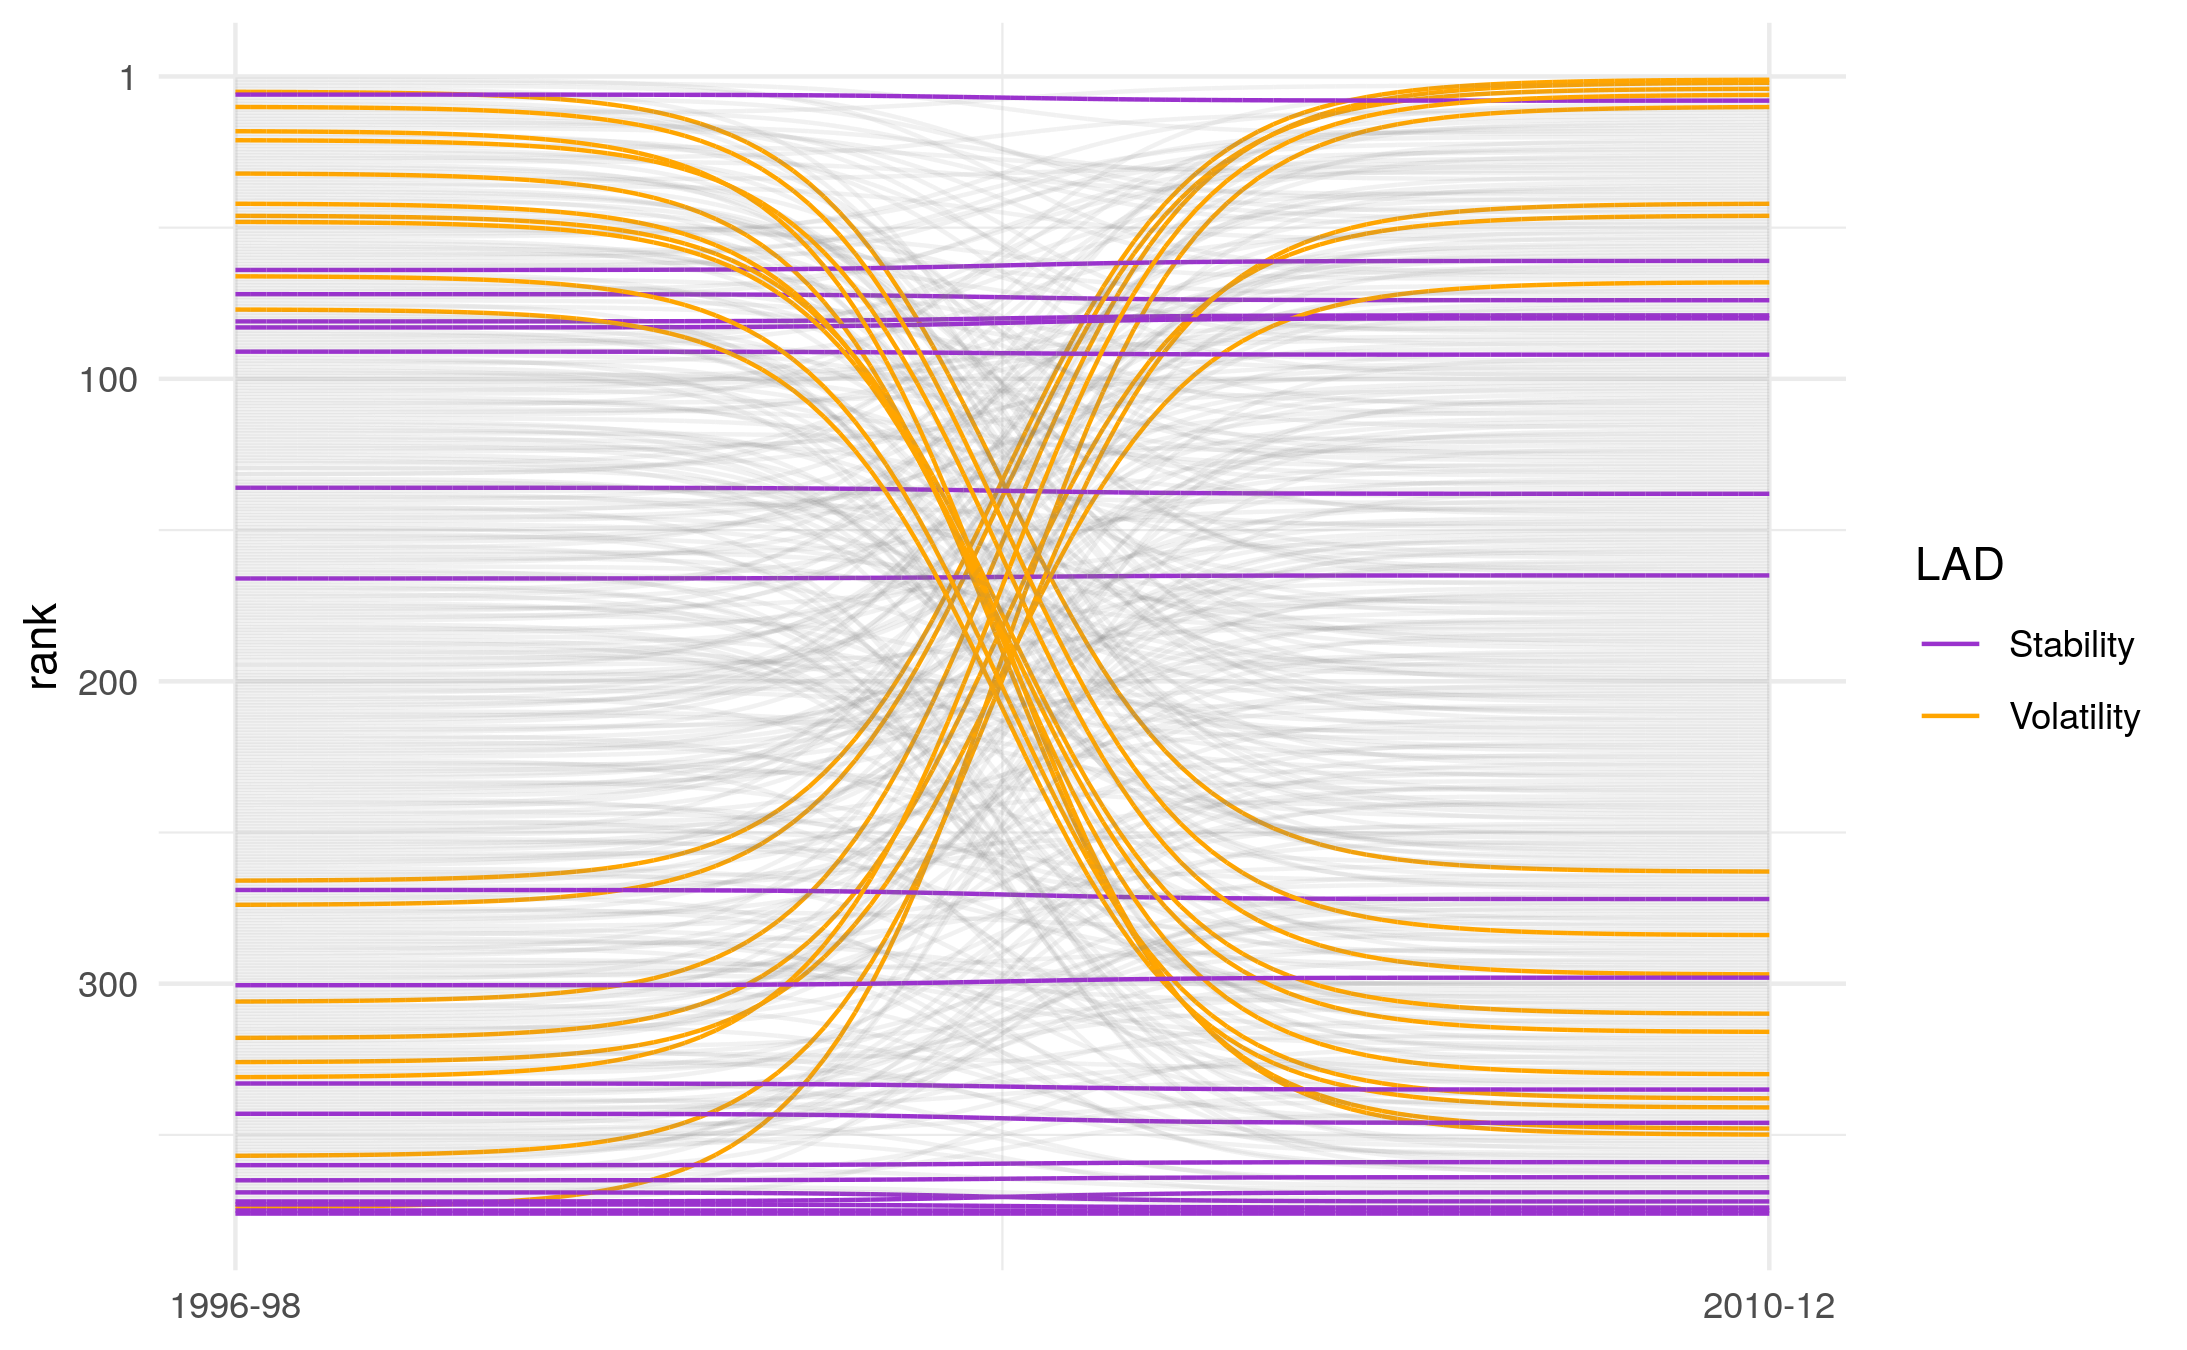
\includegraphics[width=1\textwidth,height=\textheight]{../../outputs/ranks/web_per_firm2000_2012_only0595_av.png}

}

\caption{\label{rank}Dynamics of wed diffusion (LAD)}

\end{figure}%

\subsection{Exploratory analysis}\label{exploratory-analysis}

Figures \ref{morani} and \ref{lisa} offer a first insight into whether a
neighbourhood mechanism underpins the diffusion of the Web in the UK as
they present the Moran's I and the LISA maps of website density
respectively for LAD and OA. Starting from the former, spatial
autocorrelation was higher in the beginning of the study period and then
after 2000 dropped slightly and stabilised around 0.2. This reflects the
early concentration of high website density around London, which over
time diffused as high website density clusters can be seen in other
parts of the country away from London (Figure \ref{lisa}). An almost
reverse pattern can be observed for OA. At the beginning of the study
period Moran's I was around 0.5 and it plateaued after 2000 around 0.2.
Because of the very small size of OA, at the early stages of the
diffusion of web technologies their adoption was spatially scattered.
This is reflected in the lack of any significant clusters in 1996
(Figure \ref{lisa}). Eventually, as the adoption rate increased, more
such clusters of high website density were formed and this is reflected
both in the Moran's I and the LISA maps in Figures \ref{morani} and
\ref{lisa}. A similar pattern is observed for the extended dataset (see
Figures\ref{morani10} and \ref{lisa10}). In this case, the magnitude of
spatial autocorrelation is slightly higher illustrating a stronger
spatial clustering mechanism. All in all, the exploratory spatial data
analysis advocates towards an underpinning neighbourhood mechanism and
the different scales of analysis illustrate how it evolved differently
over time. Interestingly, the magnitude of Moran's I is similar to the
ones revealed by \citet{ding2010modeling} about mobile phone adoption in
China albeit the much more detailed spatial scale of this paper.

\begin{figure}[H]

{\centering 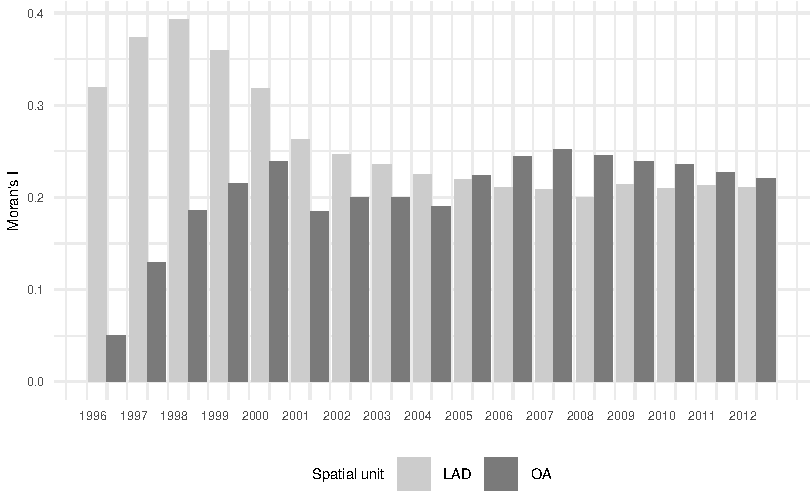
\includegraphics[width=1\textwidth,height=\textheight]{tranos2023_files/figure-pdf/morani-1.pdf}

}

\caption{\label{morani}Website density Moran's I}

\end{figure}%

\begin{figure}[H]

{\centering 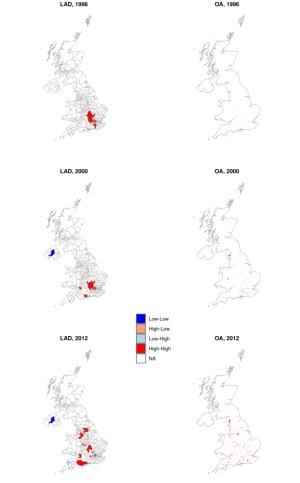
\includegraphics[width=1\textwidth,height=0.8\textheight]{tranos2023_files/figure-pdf/unnamed-chunk-6-1.pdf}

}

\caption{\label{lisa}\centering Website density LISA maps}

\end{figure}%

To illustrate whether a hierarchical process also underpins the
diffusion of web technologies, the Gini coefficient is calculated yearly
both for LAD and OA. As a metric of inequality, the Gini coefficient
demonstrates whether website density is concentrated in a small number
of LAD or OA, or whether it is more equally spread across the country.
Both scales of analysis in Figure \ref{gini} illustrate the same
picture. At the beginning of the commercial Internet, website density
was extremely unequal, or, in other words, only a few places had
websites associated with them. Inequality dropped and plateaued after
2000 for both scales. This is illustrative of a hierarchical diffusion
mechanism that led over time to a more equal spread. Interestingly, the
year 2000 is again a period of change for this diffusion mechanism as it
was for the neighbourhood process. There is a substantial difference
between the Gini coefficient magnitude for LAD and OA, but this is
expected as the very small size of OA equates to a lot of polygons
without any websites pointing to them -- for example residential OA.

\begin{figure}[H]

{\centering 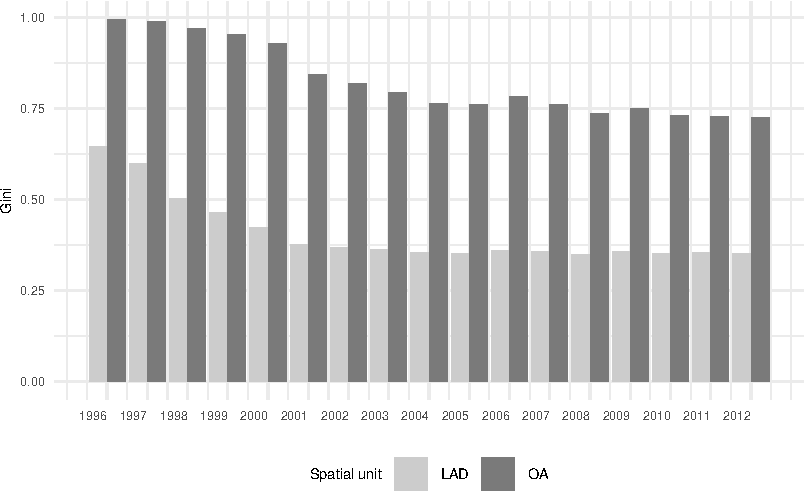
\includegraphics[width=1\textwidth,height=\textheight]{tranos2023_files/figure-pdf/gini-1.pdf}

}

\caption{\label{gini}Website density Gini coefficient}

\end{figure}%

\subsection{Modelling outputs}\label{modelling-outputs}

The next section incorporates the above mechanisms of the spatial
diffusion of the Web into a modelling framework. The aim is to use
variables depicting these spatial processes in order to predict the
diffusion of the Web as a new technology in the UK over space and time
and across different scales. Specifically, four different models are
estimated. Firstly, all the data points for the OA and LAD are utilised
in order to build two RF models and assess their capacity to predict the
adoption of the Web at the two different scales. These two models will
reveal the predictive capacity of the diffusion mechanisms and also
demonstrate how the importance of such variables changes across
different scales. The next two sets of models are again trained at these
two scales: OA and LAD. However, instead of using all the data points,
the OA and the LAD from one of the twelve UK regions are held out for
the model training. Then, the trained model is used to predict website
density for the OA or the LAD of the held-out region. This process takes
place recursively for all twelve UK regions. The regional differences in
the predictive capacity of the different samples will reveal how
dissimilar these spatial process are across regions and, importantly, at
different scales.

It needs to be highlighted here that the cross validation (CV) for all
models is spatially and temporally sensitive. Instead of using 10 random
and space- and time-agnostic folds,the \texttt{CAST} package is employed
which allows holding back data points from specific years and spatial
units and use them for testing in order to estimate the model
performance \citep{meyer2018improving}.

The models include variables that capture the three processes that the
relevant literature and the descriptive analysis highlighted. Namely,
the models capture: (i) a hierarchical mechanism with diffusion running
from main centres to secondary ones, (ii) a neighborhood mechanism
according to which diffusion first hits nearby locations, and (iii) the
rather canonical pattern of diffusion over time as reflected in the
S-shaped pattern in the cumulative level of adoption.

To capture the hierarchical mechanism the models include as predictors a
one year lag of website density in London, the largest city in the UK, a
one year lag of the website density in the nearest city and the same for
the nearest retail centre. Due to the small sizes of the retail centres,
the latter is only relevant for and included in the OA-level models. In
addition, the models include the distance to London, the nearest city
and the nearest retail centre. The underlying logic is that the level of
website adoption in a spatial unit depends on the level of the adoption
in places further up in the urban hierarchy the previous year. The
inclusion of the distance variables incorporates spatial structure into
the hierarchy argument. To depict the neighbourhood mechanism, the
website density of the neighbouring spatial units in the previous year
is employed. This is calculated using rook continuity. Again, the
underpinning rationale is that the level of web adoption within a
spatial unit depends on the level of web adoption in the neighbouring
spatial units the year before. This represents the `hitting nearby
locations first' argument. Therefore, the spatial and temporal lag of
the website density in LAD and OA is calculated. Lastly, the temporal
pattern of the cumulative adoption is captured by a time trend variable.
Hence, all four models will follow the following generic form (Eq.
\ref{model}):

\begin{align} \label{model}
Website\,Density_{t} \sim Distance\,London +
Website\,density\,London_{t-1} +\notag\\
Distance\,Nearest\,City +
Website\,density\,Nearest\,City_{t-1} +\notag\\
Distance\,Nearest\,Retail_{i} +
Website\,density\,Nearest\,Retail_{t-1} +\notag\\
W*\, Website\,density_{t-1} +\notag\\ 
year_{t}
\end{align}

To assess the predictive power of the model, three broadly utilised
metrics are employed: the coefficient of determination (\(R^2\)), mean
absolute error (MAE) and root mean square error (RMSE):

\begin{align}
R^2 = 1 - \frac{\sum_{k} (y_{k} - \hat{y_{k}})^2} {\sum_{k} (y_{k} - \overline{y_{k}})^2} \label{eq:rsquared}
\end{align}

\begin{align}
MAE = \frac{1}{N} \sum_{k = 1}^{N} |\hat{y_{k}} - y_{k}| \label{eq:mae}
\end{align}

\begin{align}
RMSE =  \sqrt{\frac{\sum_{k = 1}^{N} (\hat{y_{k}} - y_{k})^2} {N}} \label{eq:rmse}
\end{align}

\noindent \(y_{k}\) is the \(k^{th}\) observation of the dataset, which
consists of \(N\) observations in total. \(\hat{y_{k}}\) is the
\(k_{th}\) predicted value for the dependent variable and
\(\overline{y_{k}}\) is the average value of \(y\). The last two metrics
are expressed in the same units as the dependent variable -- websites
per firm for the LAD modes and the number of websites for the OA models
-- while the first one is the coefficient of determination between the
observed and the predicted values of website adoption. Regarding
\(MAE\), it is the absolute difference between the observed and the
predicted website adoption. While \(MAE\) does not penalise for large
errors, \(RSME\) does, as it is proportional to the squared difference
between the observed and the predicted trade flows. Hence larger errors
weigh more for \(RMSE\) \citep{pontius2008components}.

Table~\ref{tbl-model-metrics} presents the model performance for the
first set of models, for which all data points are employed for training
and testing via CV. The first one is trained and tested on 374 LAD and
the second on 232,296 OA, both for the 16 year period (1997-2012). The
results are remarkably good considering that the are the outcome of
space and time sensitive CV, so the the model does not suffer from
overfitting. At the LAD level the model predicts 85\% of the variation
of website density. Both error metrics indicate that the model error is
\((\frac{1}{20}, \frac{1}{30})\) of a website per firm. At the OA the
\(R^2\) drops down to 32\%. Considering its granularity, this is still a
remarkable performance. To contextualise it, the model results in a
\(MAE\) equal to one website for areas small enough to host less than
140 households. \footnote{According to the Office for National
  Statistics, 80\% of OA in England and Wales host 110-139 households,
  \href{https://www.ons.gov.uk/census/2001censusandearlier/dataandproducts/outputgeography/outputareas}{www.ons.gov.uk}.}
Because of the small size of the spatial units, the distribution is
highly skewed and a significant part of them is not linked to any
websites. In 1997 only 1\% of the UK OA were associated with at least
one website. This should not come as a surprise as this was the very
beginning of the commercial Internet and any activities with a digital
footprint were concentrated in a handful of areas. This was clearly
illustrated in Figure \ref{lisa}. At the end of the study period almost
half of the UK OA were not associated with a website. Again, given the
granularity of the data this should not come as a surprise.

\begin{longtable}[]{@{}llll@{}}
\caption{Model metrics}\label{tbl-model-metrics}\tabularnewline
\toprule\noalign{}
& \(RMSE\) & \(R^{2}\) & \(MAE\) \\
\midrule\noalign{}
\endfirsthead
\toprule\noalign{}
& \(RMSE\) & \(R^{2}\) & \(MAE\) \\
\midrule\noalign{}
\endhead
\bottomrule\noalign{}
\endlastfoot
Local Authorities & 0.028 & 0.850 & 0.019 \\
Output Areas & 3.284 & 0.320 & 1.034 \\
\end{longtable}

The results in Table~\ref{tbl-model-metrics} are robust against
different specification. As noted earlier, the data imputation process
resulted in a modest improvement of the predictive capacity of the
model. As per Table~\ref{tbl-model-metrics-no-correction} all accuracy
metrics are only slightly worst when the data imputation is not applied.
As expected, the improvement is higher for the more detailed scale of
analysis. Then, Table~\ref{tbl-model-metrics-10} presents the model
results for the extended dataset, which includes websites with up to 10
unique postcodes. While the results for the LAD are slightly less
accurate, the \(R^{2}\) of the OA model is more than double in
comparison to the base results in Table~\ref{tbl-model-metrics}. All in
all, the modelling exercise revealed how well can the three diffusion
mechanisms predict the diffusion of the Web as a new technology.
Importantly, this predictive power is highly robust against against
different scales and delineations of the diffusion of the web.

\begin{longtable}[]{@{}llll@{}}
\caption{Model metrics without data
imputation}\label{tbl-model-metrics-no-correction}\tabularnewline
\toprule\noalign{}
& \(RMSE\) & \(R^{2}\) & \(MAE\) \\
\midrule\noalign{}
\endfirsthead
\toprule\noalign{}
& \(RMSE\) & \(R^{2}\) & \(MAE\) \\
\midrule\noalign{}
\endhead
\bottomrule\noalign{}
\endlastfoot
Local Authorities & 0.032 & 0.810 & 0.019 \\
Output Areas & 5.000 & 0.205 & 1.047 \\
\end{longtable}

\begin{longtable}[]{@{}llll@{}}
\caption{Model metrics for the extended
dataset}\label{tbl-model-metrics-10}\tabularnewline
\toprule\noalign{}
& \(RMSE\) & \(R^{2}\) & \(MAE\) \\
\midrule\noalign{}
\endfirsthead
\toprule\noalign{}
& \(RMSE\) & \(R^{2}\) & \(MAE\) \\
\midrule\noalign{}
\endhead
\bottomrule\noalign{}
\endlastfoot
Local Authorities & 0.188 & 0.77 & 0.122 \\
Output Areas & 22.467 & 0.478 & 5.681 \\
\end{longtable}

Figure \ref{var.imp} plots the importance of the different predictors.
When the focus is on LAD, the website density in the nearest city, in
London and in the neighbouring LAD the year before are the most
important predictors. They are followed by the yearly trend, while the
spatial configuration as reflected in distances to London or the nearest
city only plays a minor role. This can be attributed to the relatively
coarse spatial scale of LAD. Nevertheless, all previously discussed
spatial processes are at play in the diffusion of web technologies at
the LAD level: the first two predictors depict the hierarchical
mechanism, the spatial and temporal lag of website density the
neighbourhood mechanism, and the yearly trend the time-sensitive
cumulative adoption pattern.

When the much more granular scale of OA is adopted, the picture is
almost reversed. The two most important predictors are the distance to
London and to the nearest city followed by the spatial and temporal lag
of website density and the distance to the nearest retail centre. They
still depict a hierarchical mechanism, but proximity to the different
population centres is more important than their lagged web densities in
predicting website diffusion. The neighbourhood mechanism is still
strong but less important at this scale. What is interesting is the
almost negligible role of the yearly trend and London's website density.
While the former probably illustrates the large heterogeneity in how the
Web has been adopted at this very fine scale, the latter highlights that
the importance of past web adoption rates in large population centres is
surpassed by proximity to them and spatial configuration at this scale.

The above pattern of variable importance is largely in accordance with
the models estimated for the extended dataset. A comparison with Figure
\ref{var.imp10} illustrates that the main difference is the importance
of the neighbourhood mechanism for the OA as the space and time lag of
the website density is by far the most important predictor when the
extended dataset is employed. But still, the variable importance
patterns for the two datasets are not dissimilar.

\begin{figure}[H]

{\centering 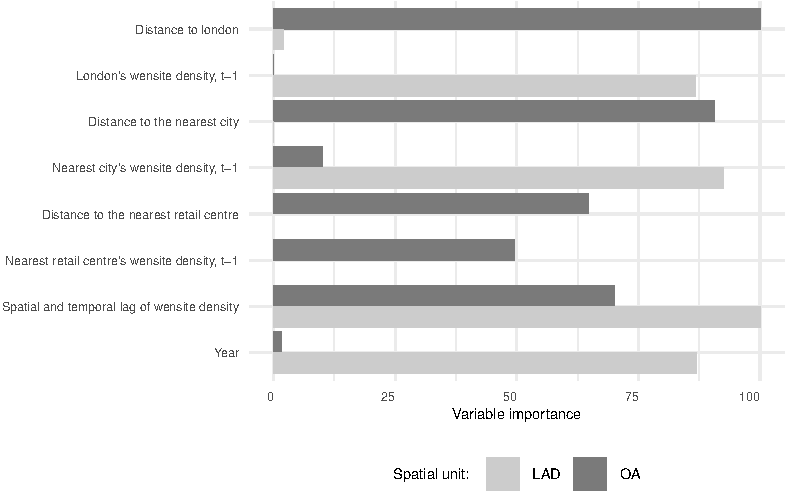
\includegraphics[width=1\textwidth,height=0.6\textheight]{tranos2023_files/figure-pdf/varimp-1.pdf}

}

\caption{\label{var.imp}Variable importance}

\end{figure}%

\begin{longtable}[]{@{}lrrrr@{}}
\caption{Regional differences\label{table.regions}}\tabularnewline
\toprule\noalign{}
Region & \(R^2\) LAD & Rank LAD & \(R^2\) OA & Rank OA \\
\midrule\noalign{}
\endfirsthead
\toprule\noalign{}
Region & \(R^2\) LAD & Rank LAD & \(R^2\) OA & Rank OA \\
\midrule\noalign{}
\endhead
\bottomrule\noalign{}
\endlastfoot
South East & 0.945 & 1 & 0.116 & 8 \\
West Midlands & 0.922 & 2 & 0.125 & 4 \\
Wales & 0.915 & 3 & 0.125 & 5 \\
Yorkshire and The Humber & 0.909 & 4 & 0.160 & 2 \\
East Midlands & 0.903 & 5 & 0.120 & 7 \\
North East & 0.896 & 6 & 0.124 & 6 \\
South West & 0.894 & 7 & 0.184 & 1 \\
London & 0.881 & 8 & 0.093 & 9 \\
East of England & 0.874 & 9 & 0.092 & 10 \\
North West & 0.837 & 10 & 0.143 & 3 \\
Scotland & 0.780 & 11 & 0.055 & 12 \\
Nortern Ireland & 0.579 & 12 & 0.060 & 11 \\
\end{longtable}

Table \ref{table.regions} presents the results of the recursive hold out
models and allows to (i) highlight the regional heterogeneity of the
spatial processes behind the diffusion of the Web, and (ii) compare this
heterogeneity across the two different scales of analysis. It
illustrates some striking similarities, but also a few significant
differences. At the top of the similarity with the rest of the country
we see West Midlands and Yorkshire and the Humber for both scales. The
web density for the LAD and OA of these regions can be very well
predicted by models trained on data for the LAD and OA of the rest of
the country. In other words, the spatial diffusion mechanisms for these
regions represent quite well the UK's average. This should not come as
as surprise given their urban structure: they both contain a large urban
centre (Birmingham and Leeds), smaller commuter towns as well as more
rural settlements. The bottom of the similarity ranking is populated by
Scotland, Northern Ireland, East of England and London for both scales.
The diffusion mechanisms for these regions diverge significantly from
the country's average and this could be attributed to rurality and
remoteness or to high levels of urbanisation and sophistication of
economic activities for the case of London and for East of England,
which contains the Cambridge area.

Still, there are three regions the spatial diffusion mechanisms of which
differ a lot between the two scales. North West and South West are very
close to the UK's average at the more granular OA scale, while the
opposite applies for South East. Interestingly, the first two regions
are well-known tourist destinations (Lake District and Cornwall-Devon)
and the exploratory analysis revealed clusters of high web density only
visible at the OA scale (Figure \ref{lisa}. Then, the South East is very
well integrated with the Greater London, hosts the broader Oxford area
-- a known hub of research excellence -- and Figure \ref{lisa} revealed
high web density clusters at the LAD level.

\section{Conclusions}\label{sec-conclusions}

This paper assessed the importance of spatial mechanisms in the
diffusion of a new technology -- the Web -- at a high level of spatial
granularity. Specifically, it assessed the capacity of the following
three spatial diffusion mechanisms in predicting website density in the
UK over space and time: (i) the hierarchical mechanism according to
which diffusion runs from main urban centres to secondary ones, (ii) the
neighborhood mechanism which highlights that diffusion first hits nearby
locations, and (iii) the rather canonical pattern of diffusion over time
as reflected in the S-shaped pattern of the cumulative level of
adoption. This is the first time that the importance of granular spatial
mechanisms for the diffusion of an intangible, digital technology is
exposed. The time period of the study is also important as it captures
the very early stages of this technology until its maturity.
Importantly, the empirical framework and the data employed here allows
to observe the active engagement with the Web that is creating and
maintaining a commercial website instead of the more passive action of
browsing webpages and accessing the Internet.

The analysis firstly illustrated how well the S-pattern of cumulative
adoption fits at the local scale of LAD. It highlighted the
heterogeneity of adoption rates between LAD -- with both more and less
expected examples -- as well as the spatial clustering of LAD with
similar adoption rates. The exploratory analysis also illustrated
instances of remarkable stability as well as volatility of the web
diffusion system that is indicative of leapfrogging. Previous research
had already indicated the long-term productivity gains of the early
adoption of such technologies \citep{tranosuk}. Then, the paper
developed a robust and novel ML modelling framework to predict website
diffusion over space and time using the three spatial diffusion
mechanisms based on space- and time-sensitive CV without suffering from
overfitting. The model revealed the remarkably good predictive capacity
of these mechanisms at both scales. For the first time, the power of
these mechanisms in predicting the diffusion of a new technology was
empirically tested, importantly, at very fine scales.

The modelling framework also revealed that the importance of these
spatial mechanisms differ across different scales. While spatial
structure as reflected in distances to different urban centres is highly
important at the OA scale, it hardly plays any role at the more coarse
LAD scale. And while the almost canonical pattern of cumulative adoption
is a key predictor at the LAD level, it only plays a small role at the
detailed OA level. Then, the analysis revealed another level of spatial
heterogeneity. While for some UK regions these spatial diffusion
mechanisms are very similar to the rest of the country, other regions
diverge significantly from the country average. Importantly, the above
results are robust against different specifications and subsets of the
data.

The paper offers a number of different contributions. Firstly, it
assesses, for the first time, the role of these spatial diffusion
mechanisms at such granular spatial scales. While previous studies had
highlighted these mechanisms
\citep{hagerstrand1968innovation, rogers2010diffusion, grubler1990rise},
their role had never been tested before at such granular scale and,
importantly, for a digital technology as weightless as the Web. The
findings talk directly to this literature
\citep[e.g.][]{beardsell1999spatial, haller2011determinants, lengyel2020role}.
More broadly, the paper offers a robust methodological framework, which
utilises novel data and modern ML algorithms and techniques to model the
diffusion of a new technology across space and time. It directly
addresses the data problem which prevented economic geographers in
engaging with diffusion studies
\citep{iso2005, kemeny2011international, zook2022mapping}. Thus, the
paper seeks to renew economic geography's interest in the diffusion of
new technologies. Current data science advances including the
availability of granular enough data and adequate methods can enable
economic geographers to reveal interesting spatial patterns of diffusion
of new technologies as this paper has demonstrated. This is important as
(i) various stakeholders are interested in predicting localised demand
for new technologies for planning purposes
\citep{leibowicz2016representing, meade2021modelling}, and (ii) the
adoption of such digital technologies is associated with economic gains
\citep{solow1957technical, aghion1990model, kemeny2011international, tranosuk, capello2024nexus}.
In addition, while most related studies focused on tangible
technologies, this paper sheds light on the diffusion of a truly
weightless digital technology that is the Web. Thus, it adds much more
granular findings to the limited related studies
\citep{sinai2004geography, haller2011determinants}. Importantly,
although the geographical focus of this paper is the UK, the empirical
framework developed here is easily transferable to other geographical
contexts.

\setcounter{section}{0}
\renewcommand{\thesection}{\Alph{section}}

\setcounter{table}{0}
\renewcommand{\thetable}{A\arabic{table}}

\setcounter{figure}{0}
\renewcommand{\thefigure}{A\arabic{figure}}

\section{Appendix}\label{appendix}

\counterwithin{figure}{section}
\counterwithin{table}{section}

\begin{figure}[H]

{\centering 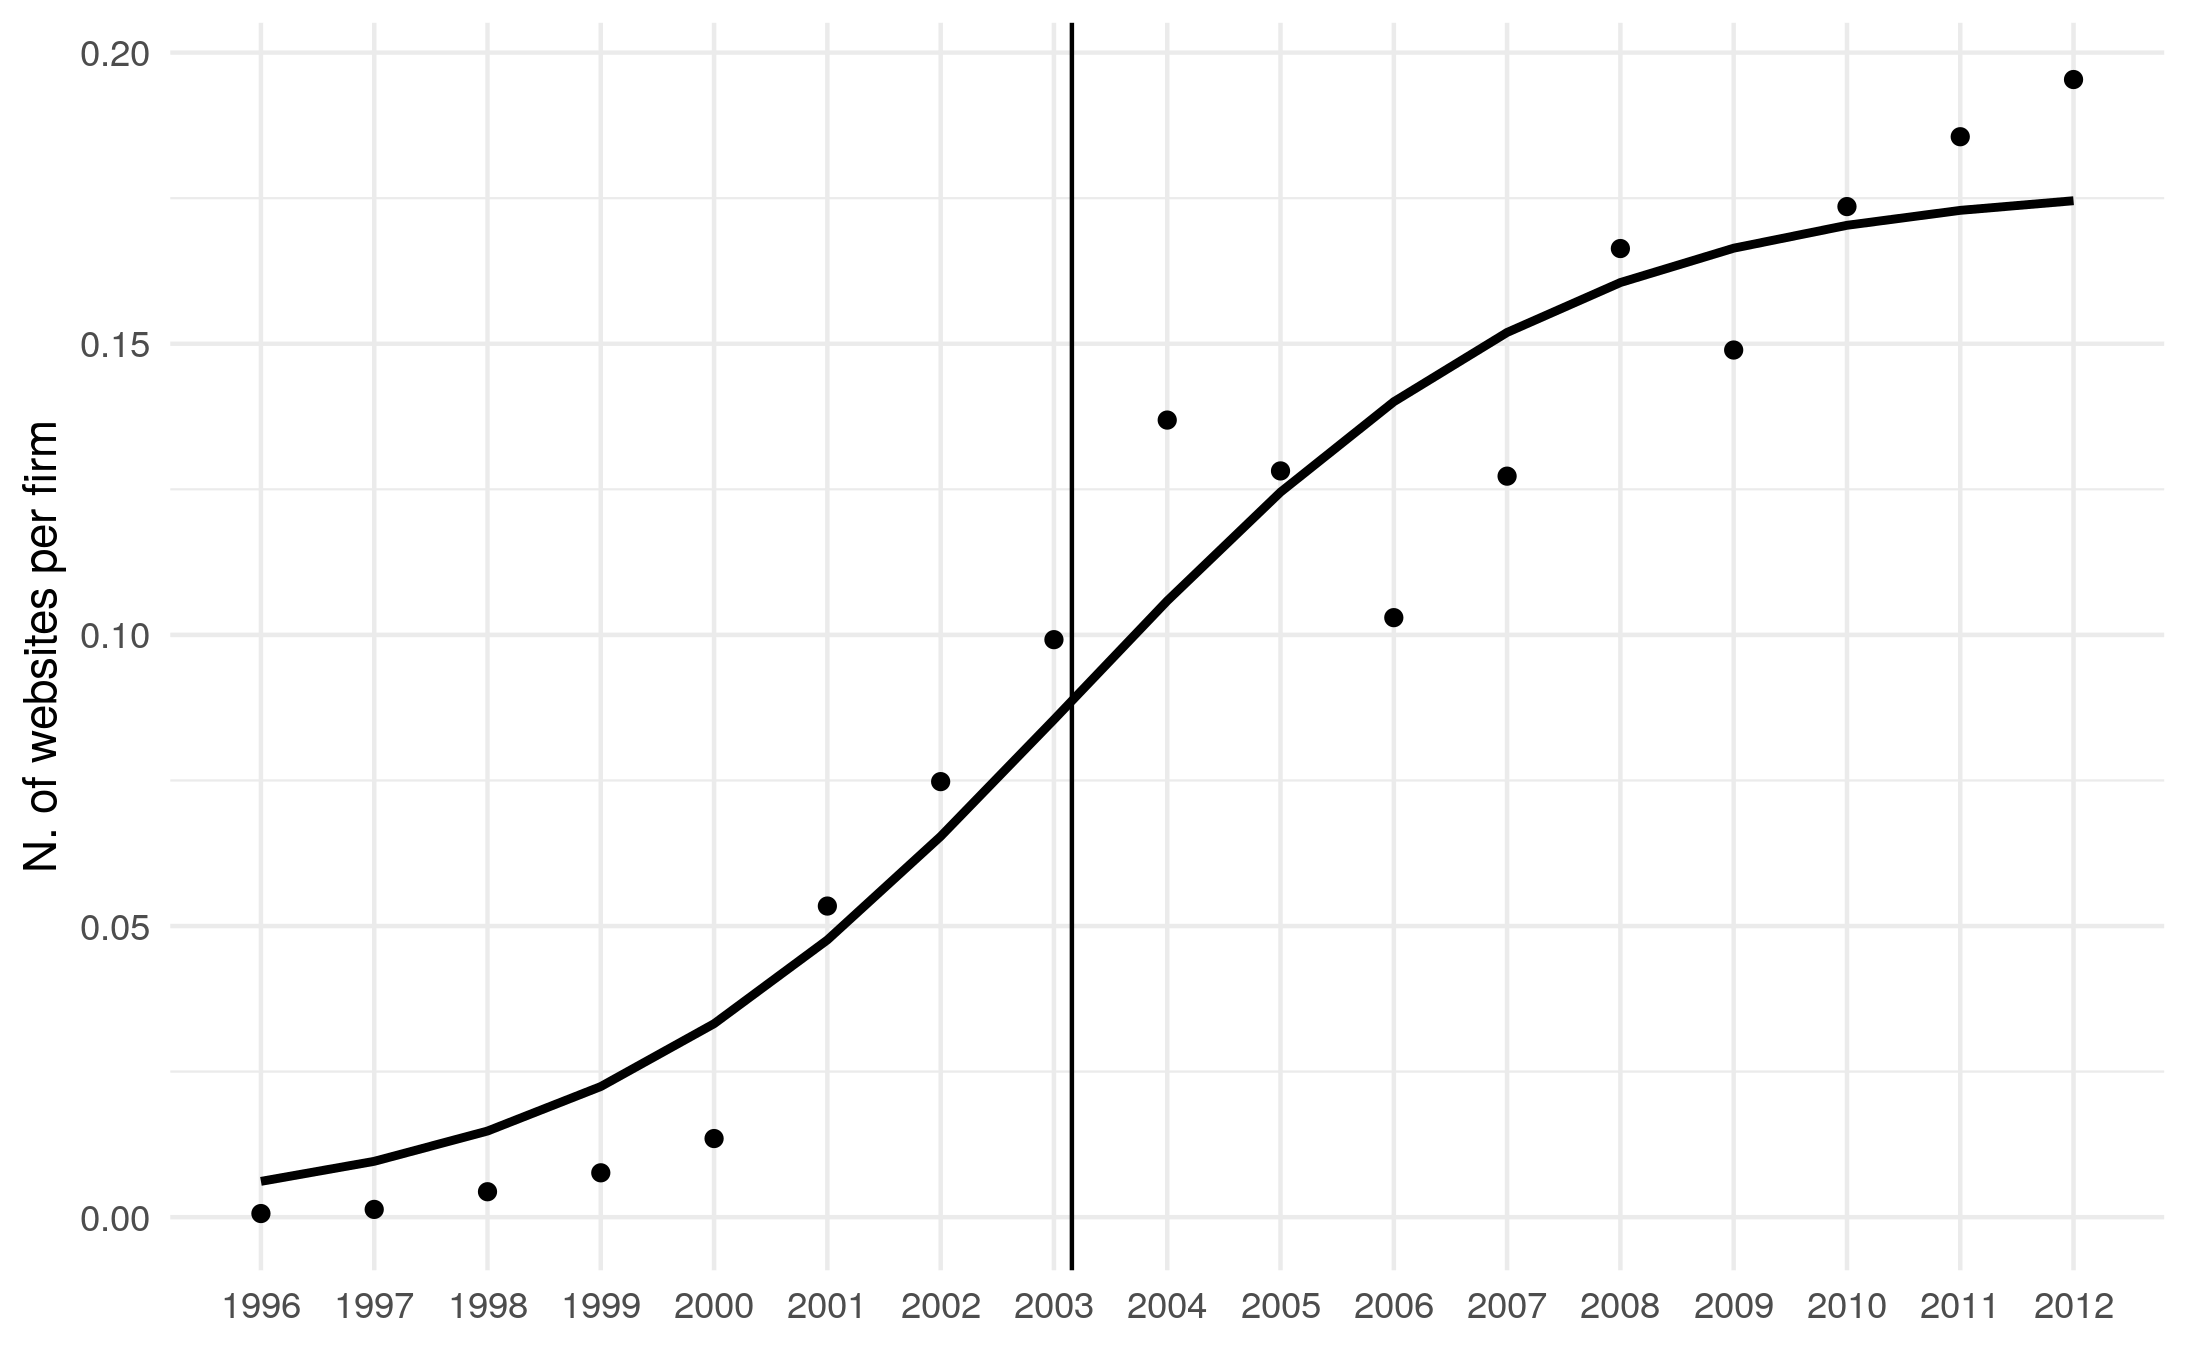
\includegraphics[width=1\textwidth,height=\textheight]{../../outputs/s/s_uk_per_firm.png}

}

\caption{\label{s_uk10}Grwoth curve, UK; up to 10 postcodes per website}

\end{figure}%

\begin{figure}[H]

{\centering 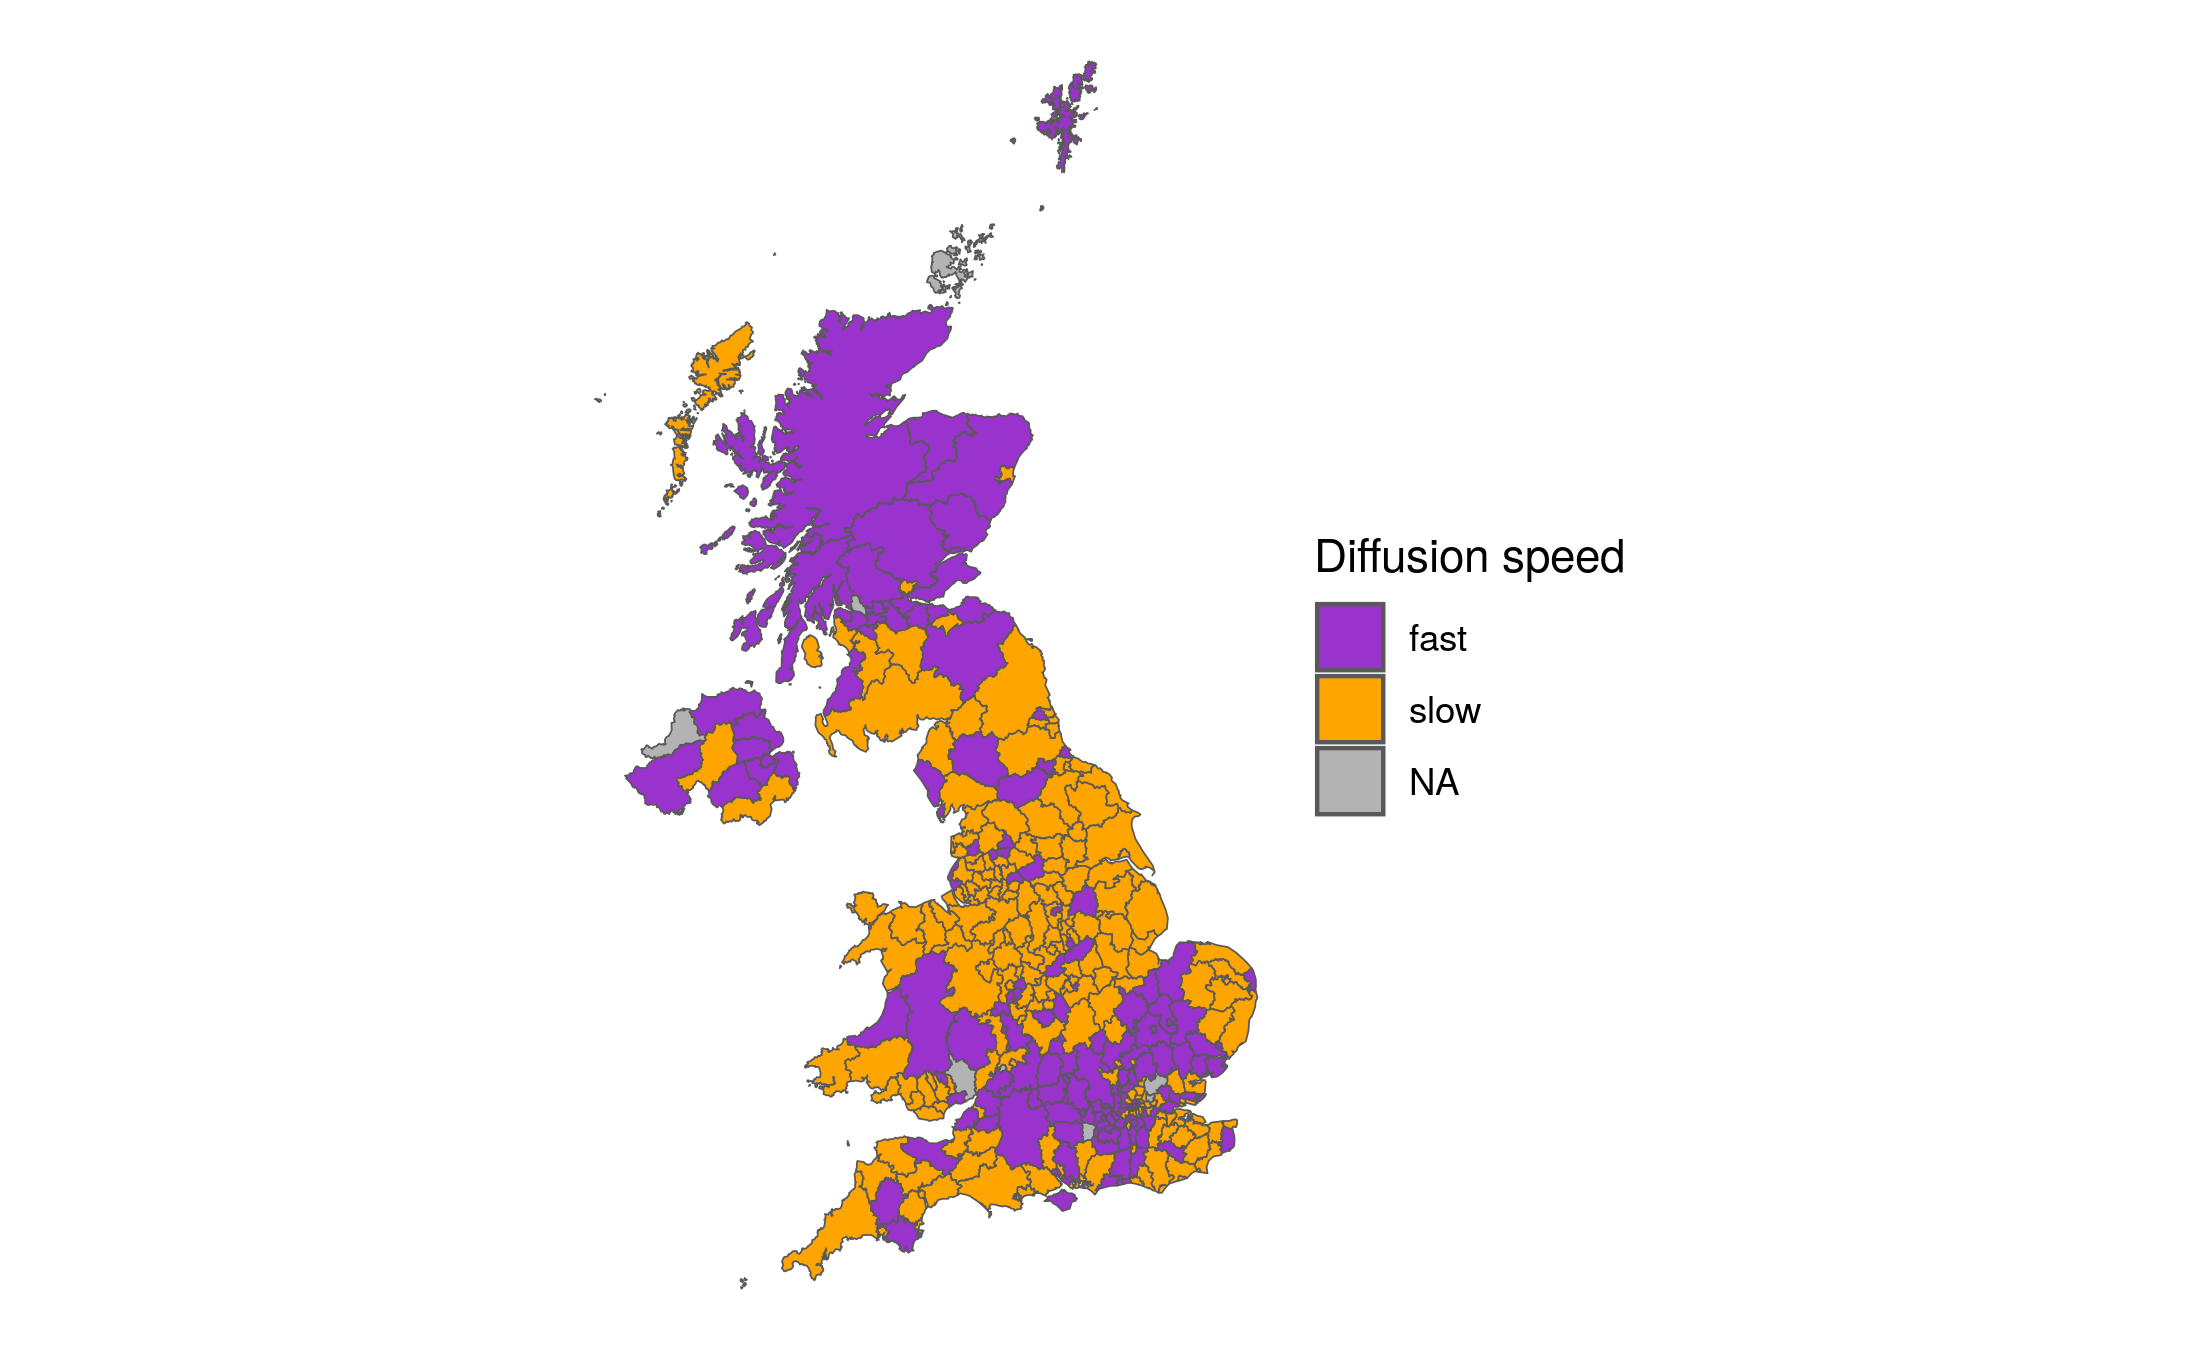
\includegraphics[width=1\textwidth,height=\textheight]{../../outputs/s/speed_map_10.png}

}

\caption{\label{s_map10}LAD adoption rates; up to 10 postcodes per
website}

\end{figure}%

\begin{figure}[H]

{\centering 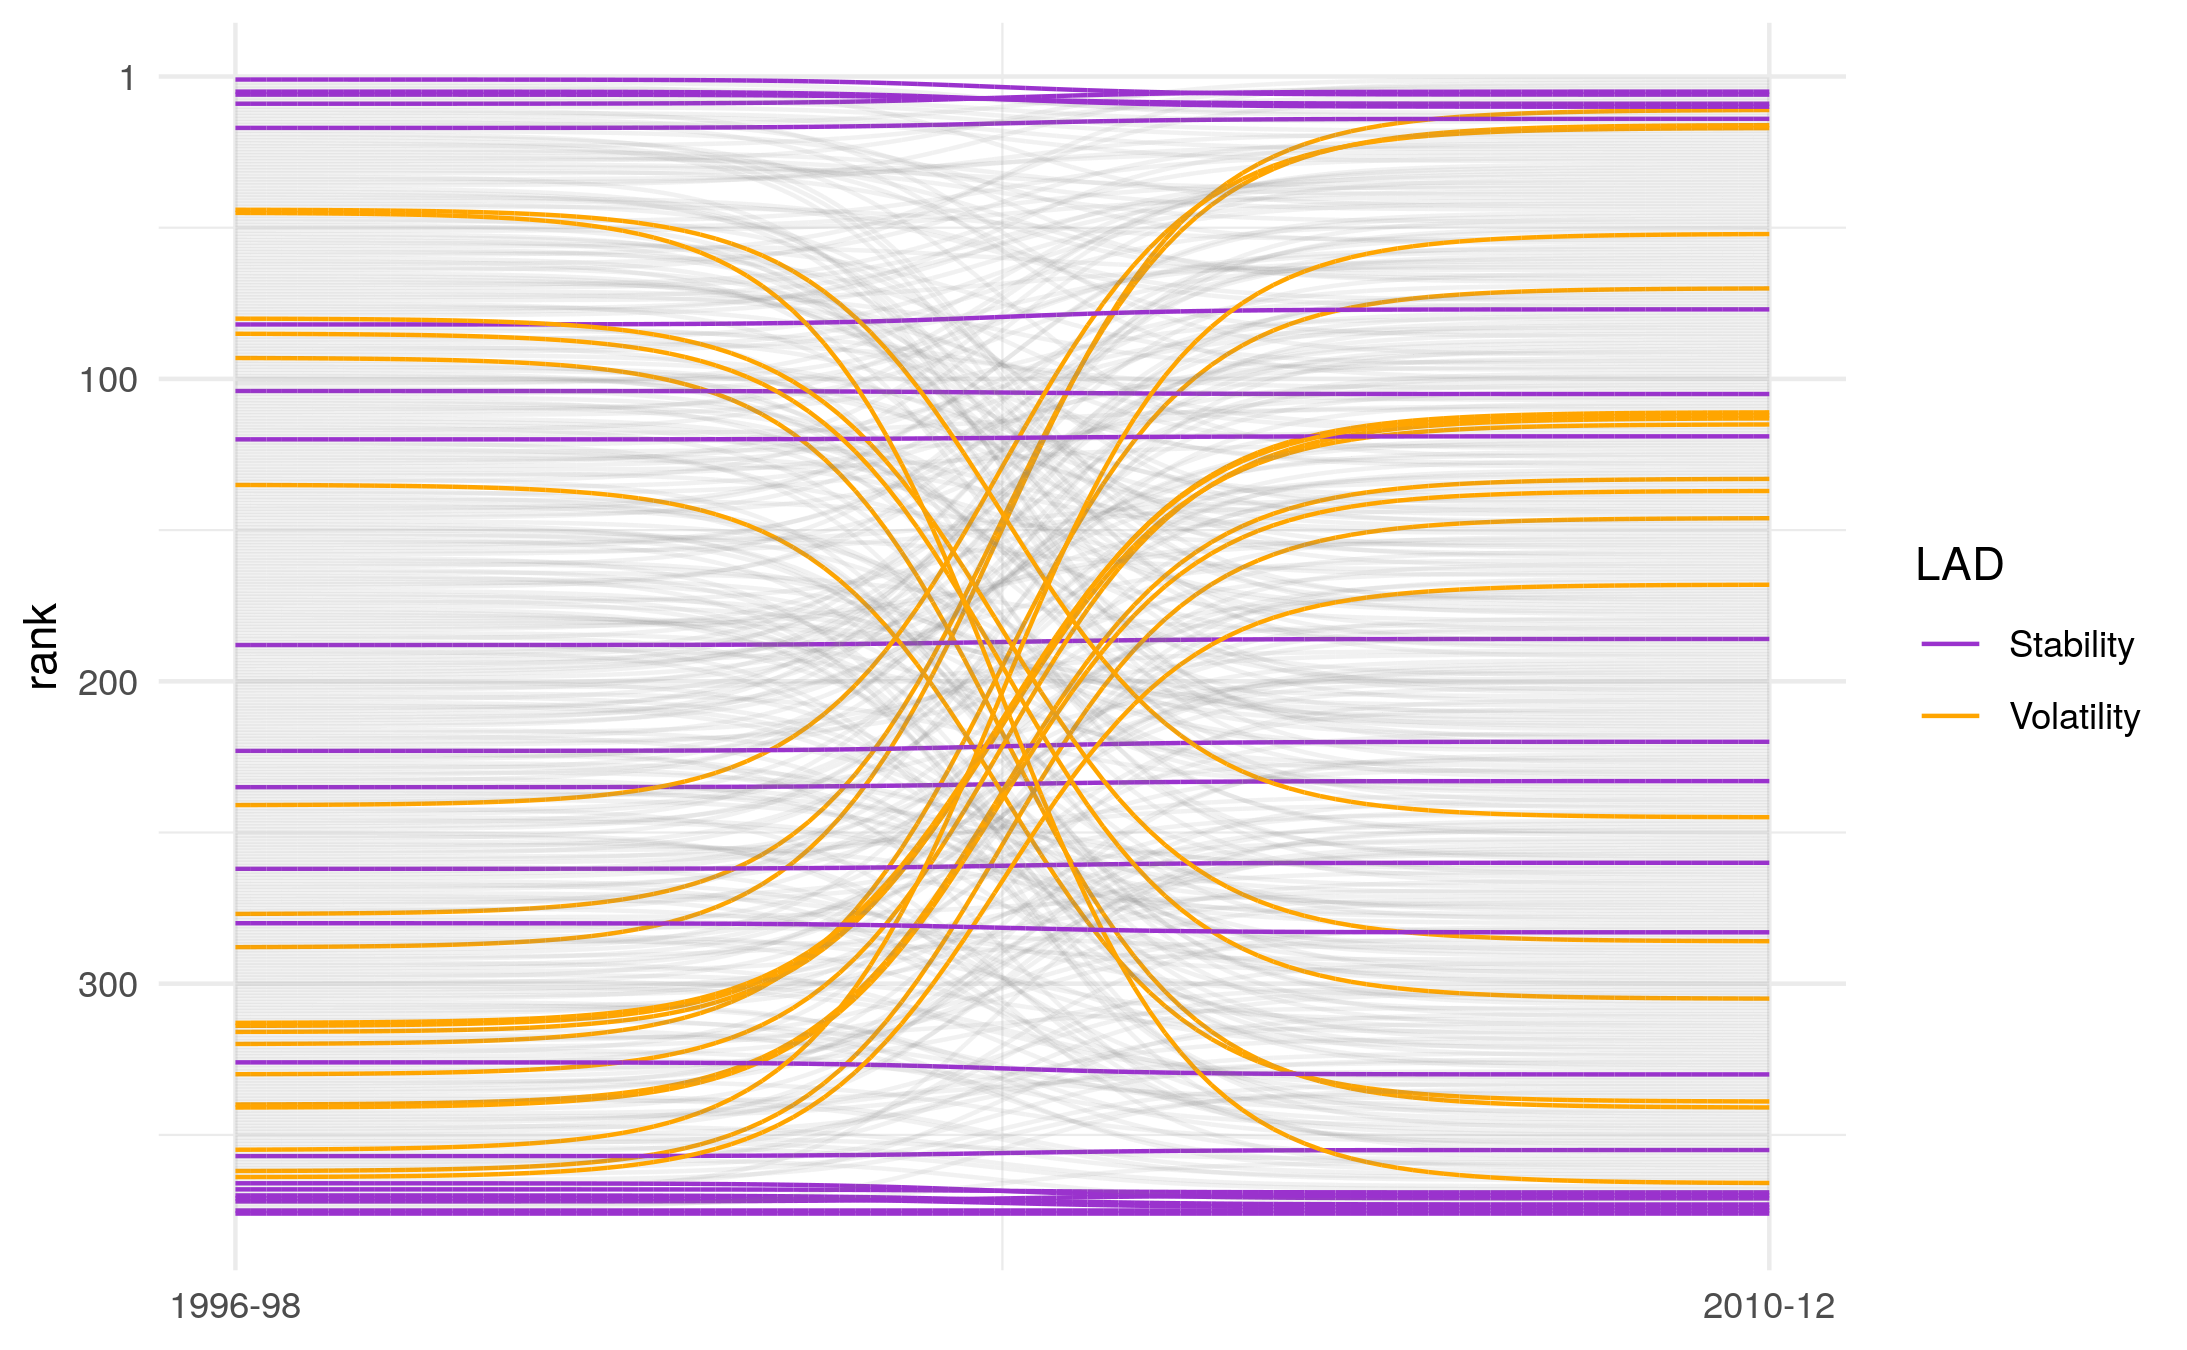
\includegraphics[width=1\textwidth,height=\textheight]{../../outputs/ranks/web_per_firm2000_2012_only0595_av_10.png}

}

\caption{\label{rank10}Dynamics of wed diffusion (LAD); up to 10
postcodes per website}

\end{figure}%

\begin{figure}[H]

{\centering 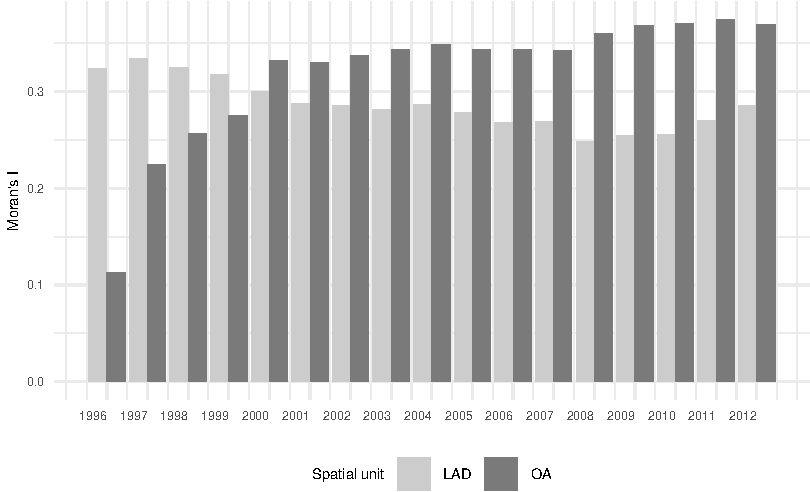
\includegraphics[width=1\textwidth,height=\textheight]{tranos2023_files/figure-pdf/morani10-1.pdf}

}

\caption{\label{morani10}Website density Moran's I; up to 10 postcodes
per website}

\end{figure}%

\begin{figure}[H]

{\centering 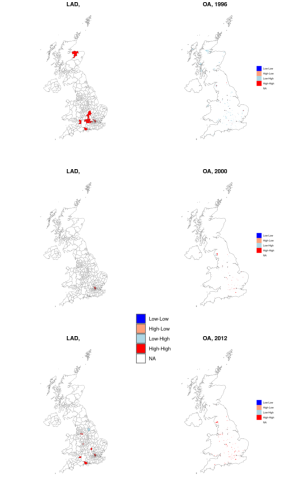
\includegraphics[width=1\textwidth,height=0.8\textheight]{tranos2023_files/figure-pdf/unnamed-chunk-10-1.pdf}

}

\caption{\label{lisa10}\centering Website density LISA maps; up to 10
postcodes per website}

\end{figure}%

\begin{figure}[H]

{\centering 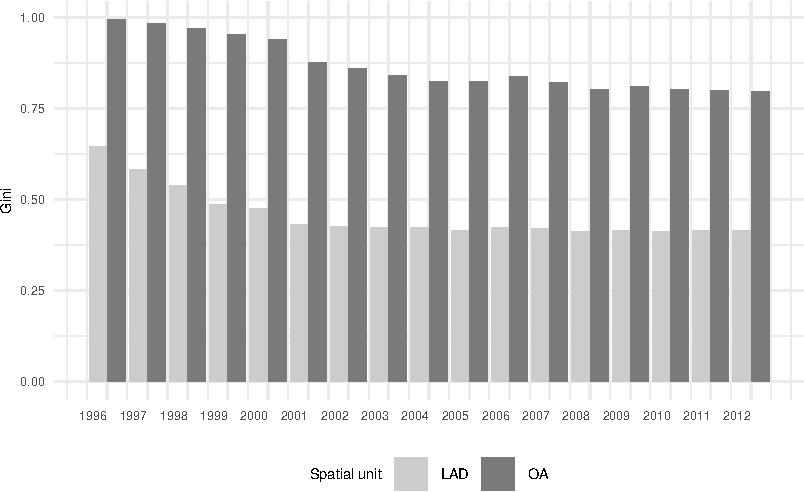
\includegraphics[width=1\textwidth,height=\textheight]{tranos2023_files/figure-pdf/gini10-1.pdf}

}

\caption{\label{gini10}Website density Gini coefficient; up to 10
postcodes per website}

\end{figure}%

\begin{figure}[H]

{\centering 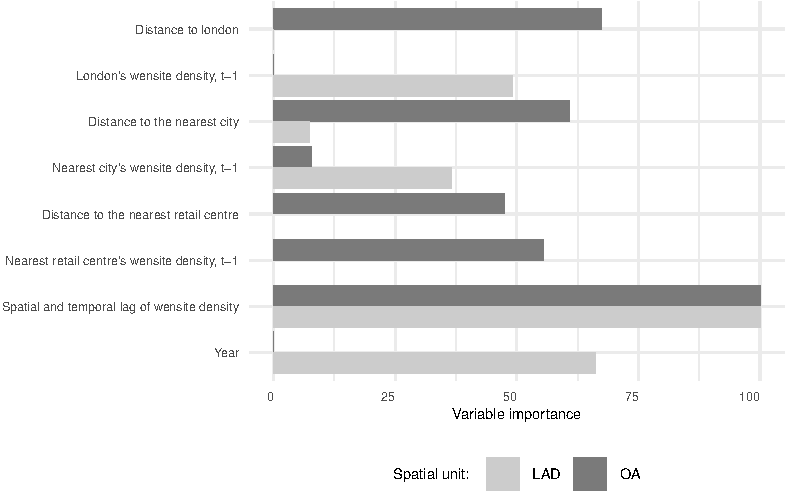
\includegraphics[width=1\textwidth,height=0.6\textheight]{tranos2023_files/figure-pdf/varimp10-1.pdf}

}

\caption{\label{var.imp10}Variable importance; up to 10 postcodes per
website}

\end{figure}%

\begin{longtable}[]{@{}lrrrr@{}}
\caption{Regional differences; up to 10 postcodes per
website\label{table.regions.no.imp}}\tabularnewline
\toprule\noalign{}
Region & \(R^2\) LAD & Rank LAD & \(R^2\) OA & Rank OA \\
\midrule\noalign{}
\endfirsthead
\toprule\noalign{}
Region & \(R^2\) LAD & Rank LAD & \(R^2\) OA & Rank OA \\
\midrule\noalign{}
\endhead
\bottomrule\noalign{}
\endlastfoot
South East & 0.947 & 1 & 0.134 & 2 \\
Wales & 0.916 & 2 & 0.131 & 3 \\
Yorkshire and The Humber & 0.906 & 3 & 0.144 & 1 \\
North East & 0.895 & 4 & 0.128 & 4 \\
West Midlands & 0.883 & 5 & 0.070 & 9 \\
East Midlands & 0.882 & 6 & 0.088 & 8 \\
East of England & 0.876 & 7 & 0.106 & 6 \\
South West & 0.864 & 8 & 0.117 & 5 \\
London & 0.805 & 9 & 0.055 & 10 \\
Scotland & 0.770 & 10 & 0.035 & 11 \\
North West & 0.664 & 11 & 0.017 & 12 \\
Nortern Ireland & 0.576 & 12 & 0.101 & 7 \\
\end{longtable}

\begin{longtable}[]{@{}
  >{\raggedright\arraybackslash}p{(\columnwidth - 10\tabcolsep) * \real{0.3186}}
  >{\raggedright\arraybackslash}p{(\columnwidth - 10\tabcolsep) * \real{0.2212}}
  >{\centering\arraybackslash}p{(\columnwidth - 10\tabcolsep) * \real{0.1416}}
  >{\centering\arraybackslash}p{(\columnwidth - 10\tabcolsep) * \real{0.1062}}
  >{\centering\arraybackslash}p{(\columnwidth - 10\tabcolsep) * \real{0.0619}}
  >{\centering\arraybackslash}p{(\columnwidth - 10\tabcolsep) * \real{0.1504}}@{}}
\caption{S-curve estiamtes for LAD; up to 10 postcodes per
website\label{table.s.lads}}\tabularnewline
\toprule\noalign{}
\begin{minipage}[b]{\linewidth}\raggedright
LAD
\end{minipage} & \begin{minipage}[b]{\linewidth}\raggedright
Region
\end{minipage} & \begin{minipage}[b]{\linewidth}\centering
\(t_0\) estimate
\end{minipage} & \begin{minipage}[b]{\linewidth}\centering
Std. error
\end{minipage} & \begin{minipage}[b]{\linewidth}\centering
\(R^2\)
\end{minipage} & \begin{minipage}[b]{\linewidth}\centering
Diffusion speed
\end{minipage} \\
\midrule\noalign{}
\endfirsthead
\toprule\noalign{}
\begin{minipage}[b]{\linewidth}\raggedright
LAD
\end{minipage} & \begin{minipage}[b]{\linewidth}\raggedright
Region
\end{minipage} & \begin{minipage}[b]{\linewidth}\centering
\(t_0\) estimate
\end{minipage} & \begin{minipage}[b]{\linewidth}\centering
Std. error
\end{minipage} & \begin{minipage}[b]{\linewidth}\centering
\(R^2\)
\end{minipage} & \begin{minipage}[b]{\linewidth}\centering
Diffusion speed
\end{minipage} \\
\midrule\noalign{}
\endhead
\bottomrule\noalign{}
\endlastfoot
Horsham & South East & 2001.423 & 0.254 & 0.950 & fast \\
Fareham & South East & 2001.443 & 0.346 & 0.925 & fast \\
Kingston upon Thames & London & 2001.513 & 0.354 & 0.933 & fast \\
Kensington and Chelsea & London & 2001.581 & 0.341 & 0.943 & fast \\
Runnymede & South East & 2001.582 & 0.266 & 0.943 & fast \\
Bracknell Forest & South East & 2001.586 & 0.324 & 0.928 & fast \\
Elmbridge & South East & 2001.656 & 0.333 & 0.932 & fast \\
Reigate and Banstead & South East & 2001.665 & 0.253 & 0.964 & fast \\
South Cambridgeshire & East of England & 2001.680 & 0.433 & 0.905 &
fast \\
Walsall & West Midlands & 2001.715 & 0.413 & 0.901 & fast \\
Surrey Heath & South East & 2001.718 & 0.333 & 0.933 & fast \\
Woking & South East & 2001.759 & 0.292 & 0.951 & fast \\
South Norfolk & East of England & 2001.874 & 0.358 & 0.931 & fast \\
City of London & London & 2001.874 & 0.499 & 0.930 & fast \\
Wokingham & South East & 2001.891 & 0.287 & 0.958 & fast \\
Reading & South East & 2001.900 & 0.318 & 0.948 & fast \\
Sevenoaks & South East & 2001.904 & 0.407 & 0.926 & fast \\
Huntingdonshire & East of England & 2001.912 & 0.402 & 0.925 & fast \\
Pendle & North West & 2001.924 & 0.407 & 0.923 & fast \\
St Albans & East of England & 2001.933 & 0.396 & 0.927 & fast \\
Perth and Kinross & NA & 2001.943 & 0.228 & 0.970 & fast \\
Bromley & London & 2001.945 & 0.396 & 0.919 & fast \\
Rushmoor & South East & 2001.962 & 0.518 & 0.912 & fast \\
Powys & NA & 2001.969 & 0.278 & 0.963 & fast \\
Swindon & South West & 2001.996 & 0.390 & 0.916 & fast \\
Chelmsford & East of England & 2002.008 & 0.545 & 0.911 & fast \\
Crawley & South East & 2002.008 & 0.379 & 0.949 & fast \\
Dumfries and Galloway & NA & 2002.012 & 0.251 & 0.967 & fast \\
Inverclyde & NA & 2002.030 & 0.330 & 0.915 & fast \\
North Hertfordshire & East of England & 2002.031 & 0.475 & 0.920 &
fast \\
Moray & NA & 2002.050 & 0.358 & 0.947 & fast \\
Orkney Islands & NA & 2002.070 & 0.283 & 0.958 & fast \\
Fife & NA & 2002.070 & 0.363 & 0.945 & fast \\
Mole Valley & South East & 2002.071 & 0.460 & 0.925 & fast \\
Guildford & South East & 2002.113 & 0.413 & 0.941 & fast \\
Buckinghamshire & South East & 2002.114 & 0.390 & 0.942 & fast \\
Cotswold & South West & 2002.116 & 0.375 & 0.946 & fast \\
Shetland Islands & NA & 2002.120 & 0.332 & 0.949 & fast \\
South Oxfordshire & South East & 2002.146 & 0.367 & 0.950 & fast \\
Watford & East of England & 2002.157 & 0.451 & 0.929 & fast \\
Aberdeenshire & NA & 2002.168 & 0.416 & 0.931 & fast \\
Southampton & South East & 2002.189 & 0.472 & 0.922 & fast \\
Mid Suffolk & East of England & 2002.196 & 0.442 & 0.922 & fast \\
Eden & North West & 2002.196 & 0.334 & 0.949 & fast \\
South Lakeland & North West & 2002.197 & 0.238 & 0.974 & fast \\
Stoke-on-Trent & West Midlands & 2002.203 & 0.419 & 0.927 & fast \\
Babergh & East of England & 2002.209 & 0.449 & 0.927 & fast \\
Bexley & London & 2002.213 & 0.493 & 0.909 & fast \\
Torbay & South West & 2002.215 & 0.374 & 0.942 & fast \\
Brentwood & East of England & 2002.219 & 0.336 & 0.936 & fast \\
Ceredigion & NA & 2002.227 & 0.241 & 0.971 & fast \\
Spelthorne & South East & 2002.232 & 0.451 & 0.933 & fast \\
Bath and North East Somerset & South West & 2002.238 & 0.402 & 0.941 &
fast \\
Falkirk & NA & 2002.245 & 0.367 & 0.938 & fast \\
Broxtowe & East Midlands & 2002.258 & 0.435 & 0.932 & fast \\
East Hertfordshire & East of England & 2002.261 & 0.453 & 0.928 &
fast \\
Stirling & NA & 2002.268 & 0.251 & 0.975 & fast \\
Ealing & London & 2002.294 & 0.523 & 0.922 & fast \\
Mid Sussex & South East & 2002.295 & 0.453 & 0.936 & fast \\
Barrow-in-Furness & North West & 2002.303 & 0.284 & 0.959 & fast \\
West Oxfordshire & South East & 2002.322 & 0.467 & 0.929 & fast \\
Sutton & London & 2002.326 & 0.544 & 0.911 & fast \\
Portsmouth & South East & 2002.356 & 0.479 & 0.921 & fast \\
Great Yarmouth & East of England & 2002.369 & 0.265 & 0.968 & fast \\
East Hampshire & South East & 2002.370 & 0.474 & 0.931 & fast \\
Wyre Forest & West Midlands & 2002.376 & 0.561 & 0.916 & fast \\
Angus & NA & 2002.378 & 0.396 & 0.939 & fast \\
Argyll and Bute & NA & 2002.427 & 0.321 & 0.962 & fast \\
Scottish Borders & NA & 2002.428 & 0.298 & 0.962 & fast \\
East Suffolk & East of England & 2002.431 & 0.533 & 0.919 & fast \\
Blackpool & North West & 2002.443 & 0.294 & 0.962 & fast \\
Cherwell & South East & 2002.448 & 0.533 & 0.923 & fast \\
Wandsworth & London & 2002.449 & 0.570 & 0.921 & fast \\
Tendring & East of England & 2002.456 & 0.456 & 0.935 & fast \\
Westminster & London & 2002.459 & 0.437 & 0.952 & fast \\
Richmond upon Thames & London & 2002.462 & 0.389 & 0.956 & fast \\
Test Valley & South East & 2002.463 & 0.553 & 0.920 & fast \\
Isle of Wight & South East & 2002.478 & 0.377 & 0.953 & fast \\
Vale of White Horse & South East & 2002.496 & 0.408 & 0.949 & fast \\
Croydon & London & 2002.510 & 0.504 & 0.927 & fast \\
Hounslow & London & 2002.521 & 0.426 & 0.952 & fast \\
Copeland & North West & 2002.524 & 0.237 & 0.971 & fast \\
Wiltshire & South West & 2002.528 & 0.450 & 0.940 & fast \\
Gwynedd & NA & 2002.536 & 0.372 & 0.954 & fast \\
Hillingdon & London & 2002.560 & 0.470 & 0.940 & fast \\
Conwy & NA & 2002.564 & 0.372 & 0.954 & fast \\
Highland & NA & 2002.566 & 0.270 & 0.972 & fast \\
Basingstoke and Deane & South East & 2002.572 & 0.461 & 0.947 & fast \\
Harrow & London & 2002.587 & 0.509 & 0.936 & fast \\
West Berkshire & South East & 2002.595 & 0.696 & 0.902 & fast \\
North Lincolnshire & Yorkshire and The Humber & 2002.596 & 0.501 & 0.933
& fast \\
East Dunbartonshire & NA & 2002.598 & 0.528 & 0.925 & fast \\
Bradford & Yorkshire and The Humber & 2002.598 & 0.613 & 0.916 & fast \\
Waverley & South East & 2002.606 & 0.512 & 0.928 & fast \\
Stroud & South West & 2002.608 & 0.559 & 0.916 & fast \\
Herefordshire, County of & West Midlands & 2002.622 & 0.388 & 0.956 &
fast \\
North Norfolk & East of England & 2002.624 & 0.422 & 0.945 & fast \\
Nottingham & East Midlands & 2002.630 & 0.531 & 0.936 & fast \\
Castle Point & East of England & 2002.645 & 0.470 & 0.936 & fast \\
North Warwickshire & West Midlands & 2002.657 & 0.380 & 0.955 & fast \\
Gravesham & South East & 2002.680 & 0.473 & 0.933 & fast \\
Lancaster & North West & 2002.692 & 0.336 & 0.963 & fast \\
West Suffolk & East of England & 2002.699 & 0.536 & 0.930 & fast \\
Stafford & West Midlands & 2002.719 & 0.499 & 0.933 & fast \\
Tunbridge Wells & South East & 2002.720 & 0.401 & 0.958 & fast \\
Oxford & South East & 2002.723 & 0.583 & 0.934 & fast \\
East Lothian & NA & 2002.731 & 0.537 & 0.927 & fast \\
Redcar and Cleveland & North East & 2002.750 & 0.509 & 0.929 & fast \\
Tamworth & West Midlands & 2002.755 & 0.551 & 0.929 & fast \\
South Hams & South West & 2002.773 & 0.422 & 0.952 & fast \\
Allerdale & North West & 2002.784 & 0.376 & 0.958 & fast \\
Central Bedfordshire & East of England & 2002.825 & 0.620 & 0.921 &
fast \\
East Cambridgeshire & East of England & 2002.843 & 0.636 & 0.927 &
fast \\
Havant & South East & 2002.853 & 0.541 & 0.932 & fast \\
South Lanarkshire & NA & 2002.874 & 0.486 & 0.938 & fast \\
Stratford-on-Avon & West Midlands & 2002.879 & 0.470 & 0.945 & fast \\
Arun & South East & 2002.882 & 0.526 & 0.938 & fast \\
Fenland & East of England & 2002.891 & 0.632 & 0.918 & fast \\
Monmouthshire & NA & 2002.893 & 0.501 & 0.935 & fast \\
Denbighshire & NA & 2002.901 & 0.457 & 0.947 & fast \\
Southend-on-Sea & East of England & 2002.903 & 0.551 & 0.932 & fast \\
High Peak & East Midlands & 2002.903 & 0.488 & 0.946 & fast \\
Pembrokeshire & NA & 2002.905 & 0.387 & 0.958 & fast \\
Malvern Hills & West Midlands & 2002.907 & 0.524 & 0.940 & fast \\
Camden & London & 2002.915 & 0.599 & 0.941 & fast \\
North Devon & South West & 2002.926 & 0.426 & 0.950 & fast \\
Wyre & North West & 2002.927 & 0.553 & 0.927 & fast \\
Darlington & North East & 2002.933 & 0.615 & 0.929 & fast \\
Swale & South East & 2002.940 & 0.447 & 0.948 & fast \\
Welwyn Hatfield & East of England & 2002.951 & 0.628 & 0.922 & fast \\
Mid Devon & South West & 2002.960 & 0.485 & 0.946 & fast \\
Lewes & South East & 2002.964 & 0.507 & 0.945 & fast \\
Dorset & South West & 2002.968 & 0.407 & 0.958 & fast \\
Brighton and Hove & South East & 2002.976 & 0.578 & 0.934 & fast \\
Braintree & East of England & 2002.978 & 0.534 & 0.938 & fast \\
Epsom and Ewell & South East & 2002.979 & 0.746 & 0.908 & fast \\
Sefton & North West & 2002.980 & 0.616 & 0.928 & fast \\
Eastleigh & South East & 2002.992 & 0.595 & 0.929 & fast \\
Craven & Yorkshire and The Humber & 2002.993 & 0.379 & 0.965 & fast \\
Hammersmith and Fulham & London & 2002.997 & 0.585 & 0.944 & fast \\
Greenwich & London & 2003.014 & 0.571 & 0.930 & slow \\
Cheltenham & South West & 2003.025 & 0.602 & 0.937 & slow \\
Worcester & West Midlands & 2003.041 & 0.659 & 0.920 & slow \\
Tower Hamlets & London & 2003.043 & 0.660 & 0.926 & slow \\
New Forest & South East & 2003.046 & 0.554 & 0.941 & slow \\
East Renfrewshire & NA & 2003.046 & 0.739 & 0.900 & slow \\
Fylde & North West & 2003.056 & 0.501 & 0.946 & slow \\
Carmarthenshire & NA & 2003.067 & 0.390 & 0.958 & slow \\
West Lancashire & North West & 2003.076 & 0.547 & 0.937 & slow \\
Hastings & South East & 2003.086 & 0.685 & 0.911 & slow \\
Carlisle & North West & 2003.111 & 0.541 & 0.934 & slow \\
Wychavon & West Midlands & 2003.115 & 0.570 & 0.935 & slow \\
Isle of Anglesey & NA & 2003.144 & 0.403 & 0.960 & slow \\
Dudley & West Midlands & 2003.150 & 0.678 & 0.925 & slow \\
Ryedale & Yorkshire and The Humber & 2003.152 & 0.380 & 0.961 & slow \\
Rother & South East & 2003.162 & 0.366 & 0.966 & slow \\
Leicester & East Midlands & 2003.167 & 0.686 & 0.924 & slow \\
Breckland & East of England & 2003.182 & 0.567 & 0.938 & slow \\
Tandridge & South East & 2003.190 & 0.747 & 0.918 & slow \\
Shropshire & West Midlands & 2003.206 & 0.621 & 0.928 & slow \\
West Devon & South West & 2003.228 & 0.489 & 0.949 & slow \\
Milton Keynes & South East & 2003.231 & 0.700 & 0.929 & slow \\
Sandwell & West Midlands & 2003.234 & 0.760 & 0.916 & slow \\
Winchester & South East & 2003.234 & 0.443 & 0.956 & slow \\
Redditch & West Midlands & 2003.238 & 0.706 & 0.923 & slow \\
Rugby & West Midlands & 2003.265 & 0.709 & 0.922 & slow \\
North Somerset & South West & 2003.278 & 0.558 & 0.939 & slow \\
West Lindsey & East Midlands & 2003.285 & 0.674 & 0.924 & slow \\
Richmondshire & Yorkshire and The Humber & 2003.286 & 0.425 & 0.958 &
slow \\
Melton & East Midlands & 2003.292 & 0.534 & 0.946 & slow \\
Chichester & South East & 2003.295 & 0.582 & 0.942 & slow \\
Torridge & South West & 2003.301 & 0.532 & 0.942 & slow \\
Dundee City & NA & 2003.303 & 0.568 & 0.939 & slow \\
South Ayrshire & NA & 2003.303 & 0.626 & 0.931 & slow \\
East Devon & South West & 2003.308 & 0.492 & 0.947 & slow \\
Bolton & North West & 2003.323 & 0.774 & 0.913 & slow \\
Hertsmere & East of England & 2003.326 & 0.726 & 0.924 & slow \\
Bournemouth, Christchurch and Poole & South West & 2003.347 & 0.662 &
0.936 & slow \\
Maldon & East of England & 2003.349 & 0.495 & 0.951 & slow \\
Barnet & London & 2003.352 & 0.766 & 0.919 & slow \\
Brent & London & 2003.389 & 0.762 & 0.925 & slow \\
Midlothian & NA & 2003.413 & 0.732 & 0.921 & slow \\
Boston & East Midlands & 2003.416 & 0.593 & 0.933 & slow \\
Scarborough & Yorkshire and The Humber & 2003.421 & 0.431 & 0.963 &
slow \\
Kirklees & Yorkshire and The Humber & 2003.435 & 0.725 & 0.925 & slow \\
Tameside & North West & 2003.441 & 0.819 & 0.907 & slow \\
Newport & NA & 2003.449 & 0.635 & 0.930 & slow \\
Glasgow City & NA & 2003.451 & 0.759 & 0.922 & slow \\
Clackmannanshire & NA & 2003.454 & 0.585 & 0.936 & slow \\
Three Rivers & East of England & 2003.458 & 0.628 & 0.947 & slow \\
Harborough & East Midlands & 2003.488 & 0.549 & 0.950 & slow \\
Rochdale & North West & 2003.496 & 0.685 & 0.937 & slow \\
Tonbridge and Malling & South East & 2003.497 & 0.710 & 0.927 & slow \\
Somerset West and Taunton & South West & 2003.502 & 0.491 & 0.955 &
slow \\
Wrexham & NA & 2003.512 & 0.553 & 0.942 & slow \\
Worthing & South East & 2003.522 & 0.622 & 0.938 & slow \\
Tewkesbury & South West & 2003.540 & 0.580 & 0.946 & slow \\
City of Edinburgh & NA & 2003.541 & 0.685 & 0.941 & slow \\
Coventry & West Midlands & 2003.592 & 0.564 & 0.948 & slow \\
Northumberland & North East & 2003.607 & 0.508 & 0.954 & slow \\
Mid and East Antrim & NA & 2003.609 & 0.893 & 0.900 & slow \\
Wigan & North West & 2003.617 & 0.755 & 0.929 & slow \\
Lichfield & West Midlands & 2003.629 & 0.625 & 0.939 & slow \\
Ashford & South East & 2003.633 & 0.535 & 0.944 & slow \\
Cornwall & South West & 2003.638 & 0.443 & 0.963 & slow \\
Mendip & South West & 2003.652 & 0.505 & 0.955 & slow \\
Stevenage & East of England & 2003.665 & 0.525 & 0.958 & slow \\
Blaenau Gwent & NA & 2003.666 & 0.643 & 0.933 & slow \\
Lincoln & East Midlands & 2003.666 & 0.634 & 0.940 & slow \\
South Somerset & South West & 2003.676 & 0.553 & 0.948 & slow \\
Charnwood & East Midlands & 2003.677 & 0.699 & 0.934 & slow \\
North Ayrshire & NA & 2003.682 & 0.607 & 0.942 & slow \\
Folkestone and Hythe & South East & 2003.684 & 0.792 & 0.905 & slow \\
Eastbourne & South East & 2003.684 & 0.697 & 0.930 & slow \\
Blackburn with Darwen & North West & 2003.685 & 0.680 & 0.938 & slow \\
Dover & South East & 2003.699 & 0.574 & 0.948 & slow \\
Adur & South East & 2003.735 & 0.551 & 0.954 & slow \\
Haringey & London & 2003.739 & 0.667 & 0.943 & slow \\
Gosport & South East & 2003.751 & 0.600 & 0.934 & slow \\
Trafford & North West & 2003.752 & 0.640 & 0.949 & slow \\
Norwich & East of England & 2003.756 & 0.742 & 0.939 & slow \\
West Lothian & NA & 2003.758 & 0.652 & 0.943 & slow \\
North East Lincolnshire & Yorkshire and The Humber & 2003.811 & 0.858 &
0.920 & slow \\
Bristol, City of & South West & 2003.828 & 0.831 & 0.928 & slow \\
Rushcliffe & East Midlands & 2003.839 & 0.591 & 0.954 & slow \\
Hinckley and Bosworth & East Midlands & 2003.857 & 0.749 & 0.934 &
slow \\
Torfaen & NA & 2003.861 & 0.841 & 0.922 & slow \\
Swansea & NA & 2003.875 & 0.650 & 0.947 & slow \\
Wolverhampton & West Midlands & 2003.882 & 0.793 & 0.931 & slow \\
Kingston upon Hull, City of & Yorkshire and The Humber & 2003.885 &
0.757 & 0.936 & slow \\
Calderdale & Yorkshire and The Humber & 2003.889 & 0.714 & 0.939 &
slow \\
North Northamptonshire & East Midlands & 2003.902 & 0.746 & 0.935 &
slow \\
Stockton-on-Tees & North East & 2003.902 & 0.955 & 0.916 & slow \\
Wealden & South East & 2003.906 & 0.736 & 0.938 & slow \\
Thanet & South East & 2003.953 & 0.667 & 0.947 & slow \\
Broadland & East of England & 2003.962 & 0.727 & 0.938 & slow \\
West Northamptonshire & East Midlands & 2003.972 & 0.736 & 0.940 &
slow \\
North Kesteven & East Midlands & 2003.976 & 0.633 & 0.942 & slow \\
Neath Port Talbot & NA & 2003.981 & 0.767 & 0.933 & slow \\
Rhondda Cynon Taf & NA & 2003.991 & 0.769 & 0.925 & slow \\
Enfield & London & 2003.992 & 0.588 & 0.954 & slow \\
East Lindsey & East Midlands & 2004.010 & 0.577 & 0.952 & slow \\
Teignbridge & South West & 2004.015 & 0.681 & 0.941 & slow \\
York & Yorkshire and The Humber & 2004.025 & 0.739 & 0.944 & slow \\
Harlow & East of England & 2004.030 & 0.803 & 0.936 & slow \\
Vale of Glamorgan & NA & 2004.033 & 0.592 & 0.951 & slow \\
Newark and Sherwood & East Midlands & 2004.034 & 0.668 & 0.946 & slow \\
Merton & London & 2004.041 & 0.932 & 0.922 & slow \\
Hambleton & Yorkshire and The Humber & 2004.065 & 0.636 & 0.953 &
slow \\
Bedford & East of England & 2004.068 & 0.852 & 0.933 & slow \\
Stockport & North West & 2004.075 & 0.757 & 0.942 & slow \\
South Ribble & North West & 2004.126 & 0.674 & 0.948 & slow \\
Uttlesford & East of England & 2004.144 & 0.905 & 0.926 & slow \\
Rossendale & North West & 2004.160 & 0.976 & 0.923 & slow \\
Oldham & North West & 2004.162 & 0.801 & 0.938 & slow \\
Sheffield & Yorkshire and The Humber & 2004.189 & 0.770 & 0.944 &
slow \\
Ribble Valley & North West & 2004.204 & 0.718 & 0.945 & slow \\
Maidstone & South East & 2004.222 & 0.854 & 0.932 & slow \\
Cheshire West and Chester & North West & 2004.234 & 0.742 & 0.947 &
slow \\
Thurrock & East of England & 2004.241 & 0.841 & 0.924 & slow \\
Telford and Wrekin & West Midlands & 2004.241 & 1.024 & 0.917 & slow \\
Cardiff & NA & 2004.246 & 0.823 & 0.937 & slow \\
County Durham & North East & 2004.250 & 0.626 & 0.953 & slow \\
Plymouth & South West & 2004.252 & 0.785 & 0.934 & slow \\
Bridgend & NA & 2004.256 & 0.547 & 0.956 & slow \\
Rotherham & Yorkshire and The Humber & 2004.273 & 0.722 & 0.938 &
slow \\
Hyndburn & North West & 2004.298 & 0.881 & 0.932 & slow \\
Newcastle upon Tyne & North East & 2004.305 & 0.906 & 0.932 & slow \\
Wakefield & Yorkshire and The Humber & 2004.314 & 0.905 & 0.923 &
slow \\
Havering & London & 2004.345 & 0.822 & 0.938 & slow \\
South Kesteven & East Midlands & 2004.353 & 1.026 & 0.915 & slow \\
Canterbury & South East & 2004.354 & 0.602 & 0.960 & slow \\
Broxbourne & East of England & 2004.363 & 0.817 & 0.944 & slow \\
Peterborough & East of England & 2004.382 & 0.937 & 0.932 & slow \\
Redbridge & London & 2004.411 & 1.028 & 0.925 & slow \\
Bury & North West & 2004.431 & 0.735 & 0.953 & slow \\
Harrogate & Yorkshire and The Humber & 2004.433 & 0.971 & 0.927 &
slow \\
Birmingham & West Midlands & 2004.435 & 1.182 & 0.912 & slow \\
South Tyneside & North East & 2004.446 & 0.636 & 0.948 & slow \\
Chorley & North West & 2004.462 & 1.093 & 0.913 & slow \\
North East Derbyshire & East Midlands & 2004.483 & 0.703 & 0.953 &
slow \\
Lambeth & London & 2004.485 & 0.958 & 0.937 & slow \\
Doncaster & Yorkshire and The Humber & 2004.496 & 0.672 & 0.953 &
slow \\
South Gloucestershire & South West & 2004.499 & 0.881 & 0.937 & slow \\
Caerphilly & NA & 2004.499 & 0.819 & 0.938 & slow \\
East Staffordshire & West Midlands & 2004.501 & 1.132 & 0.910 & slow \\
North Tyneside & North East & 2004.509 & 0.864 & 0.933 & slow \\
South Holland & East Midlands & 2004.534 & 0.851 & 0.941 & slow \\
Gateshead & North East & 2004.535 & 0.869 & 0.934 & slow \\
St.~Helens & North West & 2004.542 & 1.097 & 0.923 & slow \\
Flintshire & NA & 2004.549 & 0.764 & 0.951 & slow \\
Selby & Yorkshire and The Humber & 2004.549 & 0.716 & 0.947 & slow \\
Belfast & NA & 2004.556 & 1.332 & 0.906 & slow \\
Sedgemoor & South West & 2004.613 & 0.540 & 0.966 & slow \\
Exeter & South West & 2004.617 & 0.964 & 0.936 & slow \\
South Derbyshire & East Midlands & 2004.629 & 0.934 & 0.938 & slow \\
Derbyshire Dales & East Midlands & 2004.668 & 0.648 & 0.963 & slow \\
East Riding of Yorkshire & Yorkshire and The Humber & 2004.683 & 0.728 &
0.955 & slow \\
Basildon & East of England & 2004.691 & 1.067 & 0.925 & slow \\
Barking and Dagenham & London & 2004.800 & 1.198 & 0.916 & slow \\
Causeway Coast and Glens & NA & 2004.834 & 1.024 & 0.928 & slow \\
North Lanarkshire & NA & 2004.839 & 0.878 & 0.945 & slow \\
Chesterfield & East Midlands & 2004.887 & 1.173 & 0.927 & slow \\
Newcastle-under-Lyme & West Midlands & 2004.933 & 1.172 & 0.925 &
slow \\
East Ayrshire & NA & 2004.934 & 1.280 & 0.903 & slow \\
Nuneaton and Bedworth & West Midlands & 2004.956 & 0.950 & 0.941 &
slow \\
Blaby & East Midlands & 2004.959 & 1.059 & 0.929 & slow \\
Leeds & Yorkshire and The Humber & 2004.979 & 0.836 & 0.956 & slow \\
Erewash & East Midlands & 2004.987 & 0.939 & 0.944 & slow \\
Bassetlaw & East Midlands & 2004.998 & 0.982 & 0.944 & slow \\
Hackney & London & 2005.026 & 1.157 & 0.934 & slow \\
Barnsley & Yorkshire and The Humber & 2005.055 & 0.912 & 0.942 & slow \\
Amber Valley & East Midlands & 2005.105 & 1.017 & 0.941 & slow \\
Colchester & East of England & 2005.144 & 1.250 & 0.927 & slow \\
Ashfield & East Midlands & 2005.176 & 1.073 & 0.942 & slow \\
Wirral & North West & 2005.184 & 1.084 & 0.939 & slow \\
Knowsley & North West & 2005.186 & 1.160 & 0.923 & slow \\
Windsor and Maidenhead & South East & 2005.195 & 1.746 & 0.902 & slow \\
Bromsgrove & West Midlands & 2005.494 & 1.144 & 0.941 & slow \\
Liverpool & North West & 2005.526 & 1.276 & 0.936 & slow \\
Staffordshire Moorlands & West Midlands & 2005.583 & 1.426 & 0.924 &
slow \\
Islington & London & 2005.970 & 1.223 & 0.955 & slow \\
Warrington & North West & 2006.015 & 1.387 & 0.942 & slow \\
Newham & London & 2006.078 & 1.908 & 0.907 & slow \\
Bolsover & East Midlands & 2006.188 & 1.143 & 0.957 & slow \\
Lisburn and Castlereagh & NA & 2006.193 & 1.970 & 0.903 & slow \\
Manchester & North West & 2006.449 & 1.434 & 0.950 & slow \\
Sunderland & North East & 2006.479 & 1.679 & 0.928 & slow \\
South Staffordshire & West Midlands & 2006.490 & 1.837 & 0.922 & slow \\
Rutland & East Midlands & 2006.529 & 0.986 & 0.967 & slow \\
Cannock Chase & West Midlands & 2006.700 & 2.231 & 0.917 & slow \\
Mansfield & East Midlands & 2006.889 & 1.579 & 0.946 & slow \\
Ards and North Down & NA & 2006.947 & 2.485 & 0.907 & slow \\
Halton & North West & 2007.069 & 0.932 & 0.967 & slow \\
Burnley & North West & 2007.372 & 2.286 & 0.919 & slow \\
Middlesbrough & North East & 2010.074 & 5.297 & 0.900 & slow \\
Isles of Scilly & South West & 2012.163 & 4.257 & 0.953 & slow \\
\end{longtable}


\renewcommand\refname{References}
  \bibliography{bibliography}



\end{document}
